\chapter {Introducción}
\label{sec:intro}
\rmfamily
El proyecto debe cubrir la necesidad de recursos Software en el lenguaje musical, o antiguamente conocido como solfeo, siendo esta una asignatura primordial para las enseñanzas en cualquier centro educativo donde se aprenda a tocar cualquier instrumento mediante el proyecto "Definición y desarrollo de Solución Informática para el aprendizaje del lenguaje musical".

Para esto, se ha realizado una investigación en el marco musical con la premisa de averiguar necesidades de profesorado y alumnado y obtener ejemplos de cualquier herramienta informática ya creada para las enseñanzas de los centros mencionados, dicha investigación comenzará alrededor de los centros que enseñen esta asignatura mediante una serie de objetos (como encuestas o entrevistas) que serán de gran utilidad a la hora de realizar una mejor cobertura a nivel de Software a través de este mismo proyecto o futuros proyectos que se basen en este estudio.

Tras ello, se continuará la investigación mediante un estudio bibliográfico, en el cual, se obtendrá más información vital para la solución requerida, de esta forma, se tendrán dos grandes bloques de información, los cuales, serán comparados mediante la percepción propia como antiguo alumno de la asignatura. 

Gracias a todo este trabajo se podrán definir una solución informática que cubra las necesidades detectadas y, que posteriormente, será desarrollada.

\chapter {Objetivos}

El objetivo principal sería, por tanto, \textbf {resolver la problemática en relación a la falta de recursos informáticos enfocados a la enseñanza del lenguaje musical}. Para alcanzar dicho objetivo, se deben cumplir, a su vez, los siguientes subobjetivos:
\begin{itemize}

\item \textbf {Entender las necesidades de profesores y alumnos de lenguaje musical.}
\item \textbf {Aprender sobre la relación existente entre la informática y el lenguaje musical.}
\item \textbf {Definir una solución informática que cubra las necesidades detectadas.}
\item \textbf {Diseñar y desarrollar una de las soluciones.}
\item \textbf {Llevar a cabo el proceso de desarrollo con tecnologías totalmente.}
\end{itemize}
\chapter {Marco teórico}
\label{sec:marco}
\section {Contexto}

El lenguaje musical, como se ha mencionado, es una asignatura enseñada en la gran mayoría de centros de estudio de la música, pero, como su propio nombre indica, también es un lenguaje o "idioma" (es por ello que la asignatura en la que se estudia tiene el mismo nombre).

Al igual que otros idiomas a la hora de comunicarse redactada y verbalmente, es el método que se usa para transmitir algo mediante la música. Por tanto, al igual que existen las letras, las palabras o los distintos signos de puntuación, en este caso, se tendrán una serie de elementos para establecer la comunicación:

\begin{figure}[h]
    \centering
    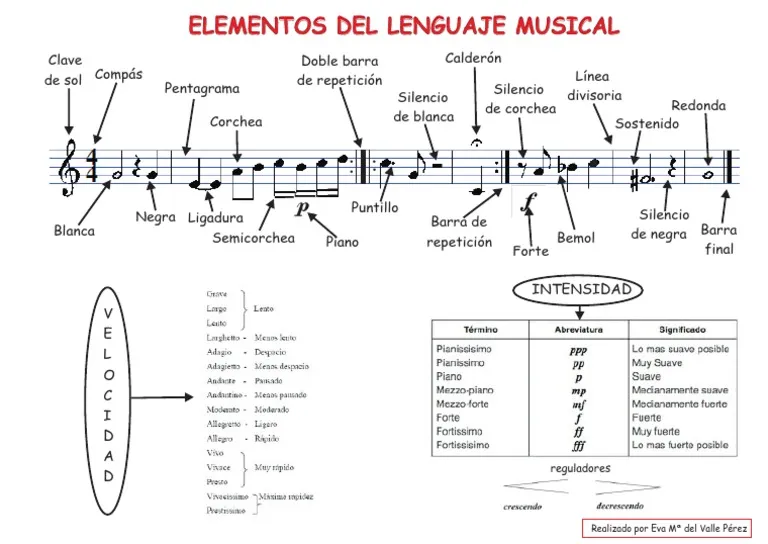
\includegraphics[width=1\linewidth]{Figuras/image.png}
    \caption{Elementos del lenguaje musical}
    \label{fig:enter-label}
\end{figure}
\newpage
Para aprender a utilizar todos estos elementos tanto de forma escrita como oral es necesario estudiar las siguientes cuatro ramas:

\begin{itemize}
\item \textbf {Ritmo:} Es la parte del lenguaje musical que consiste en la enseñanza de la lectura de partituras con fluidez.

\item \textbf {Entonación:} Esta rama se encarga del estudio de la entonación de partituras con fluidez.

\item \textbf {Audición:} La audición es otra de las ramas del lenguaje musical y en ella se entrena el oído para ser capaz de entender cualquier fragmento musical con el fin de poder plasmarlo (principalmente de forma escrita).

\item \textbf {Teoría:} Por último, existe una parte en el lenguaje musical que consiste en la enseñanza teórica de la misma.
\end{itemize}

A través del estudio de las anteriores, se puede llegar a conseguir un dominio completo en el uso del lenguaje musical, por lo tanto, es importante tenerlas en cuenta de cara a la construcción de una solución.

Otro aspecto fundamental es la diferenciación entre escuelas de música y conservatorios. Los primeros, habitualmente, están gestionados por asociaciones y/o pequeñas empresas y, aunque pueden beneficiarse de alguna subvención local, son por tanto privados lo que significa que cada uno puede tener una manera muy diferente de enfocar la asignatura por lo que las necesidades pueden ser diferentes, en cambio, los conservatorios son públicos, de esta forma, la manera de enseñar la asignatura será muy parecida entre todos los centros.

\section {Relación entre la informática y el lenguaje musical}

Para entender el dominio del proyecto es primordial entender su relación con la informática, en este caso, con el objetivo de definir y construir una solución. A priori, puede parecer que el lenguaje musical y la informática sean dos ámbitos bastante alejados, pero en el primero se ha detectado un grave problema y es el tedioso método de enseñanza que tiene mediante lecciones magistrales que provocan una sensación de aburrimiento en el alumnado que, a su vez, conlleva a una gran falta de interés por parte de los mismos y que desemboca en un aprendizaje lento. Es por ello, que la ingeniería podría tener un buen impacto al ser su principal objetivo resolver los problemas, en este caso, a través de la informática.

\chapter {Investigación}

\section {Introducción}

Como se ha mencionado, se ha llevado a cabo una investigación alrededor de los centros de enseñanza musical, para ello, se han diseñado una serie de encuestas y entrevistas enfocadas tanto al profesorado como al alumnado de cara a entender sus necesidades. Lo primero que se ha tenido en cuenta son esas diferencias que pueda haber entre los centros públicos y privados, por lo que ha sido necesario visitar dos entornos diferentes, el Real Conservatorio Profesional de Música de Almería (público) y la Escuela de Música de Huércal de Almería (privado). 

En ambos centros se ha tenido cita con un profesor de la asignatura para tener una entrevista y entregarles una encuesta para que más tarde fueran devueltas y rellenas por todo el alumnado al cargo de los profesores mencionados. Tras ello se analizarán todas las respuestas y se compararán las del público con las del privado (tanto las entrevistas como las encuestas) que, como se podrá apreciar más tarde, las preguntas también tendrán ligeras modificaciones entre las cuestionadas en un centro y otro.

A través de este método, se podrán conocer las herramientas informáticas usadas actualmente, lo cual será de ayuda en el estudio bibliográfico y así poder poner el foco sobre las funcionalidades más interesantes. 

Por último, se extraerán también del análisis las necesidades del profesorado y el alumnado actuales, lo cual servirá para poder definir correctamente las posibles soluciones a la problemática.

\newpage

\section {Análisis y comparación de las respuestas de los profesores}

Las preguntas y respuestas realizadas en las entrevistas de ambos profesores han sido las siguientes:

\begin{figure}[h]
    \centering
    \subfloat[Profesor del conservatorio]{
        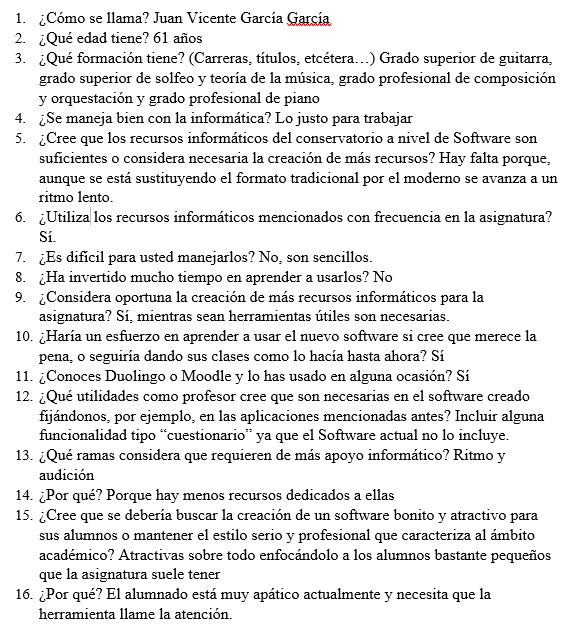
\includegraphics[width=0.5\linewidth]{Figuras/entrevistaC.png}
    }
    \subfloat[Profesora de la escuela de música]{
        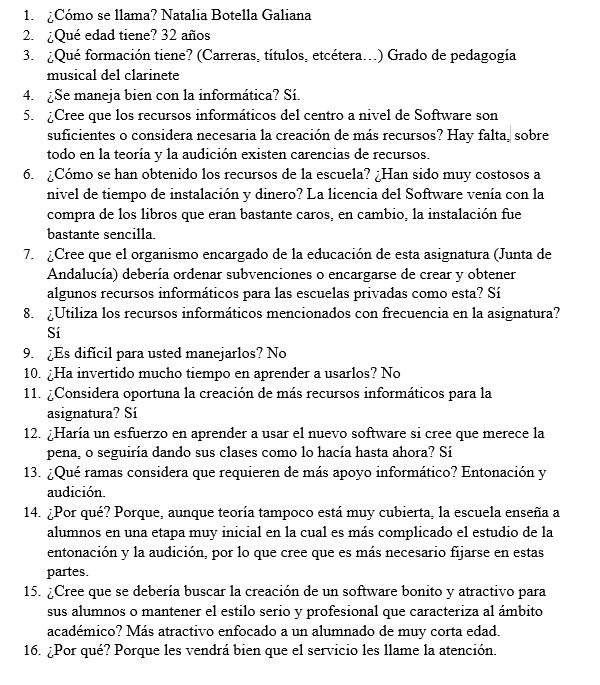
\includegraphics[width=0.5\linewidth]{Figuras/entrevistaE.png}
    }
    \caption{Entrevistas}
    \label{fig:enter-label}
\end{figure}

En primer lugar, se puede apreciar que se han cambiado dos preguntas entre entrevista, esto es debido a que en el ámbito privado era importante obtener información relativa a la obtención de los recursos (lo cual está más claro en lo público) y, por contraparte, era interesante preguntar sobre herramientas de la Junta como Moodle al profesor del Conservatorio (Duolingo era para dar un ejemplo diferente). Tras ver estas respuestas se pueden concluir los siguientes aspectos:

\begin{enumerate}
\item A pesar de la diferencia de edad, ambos coinciden en que tienen la habilidad y predisposición suficiente para aprender a usar un nuevo servicio informático siempre y cuando sea intuitivo debido a la escasez y necesidad de recursos en ambos sectores (público y privado).

\item Ambos le dan bastante uso a los recursos que tienen actualmente.
 \newpage
\item También coinciden que la audición está menos cubierta, en cambio, en lo público parece que en el ritmo existe una mayor necesidad y en lo privado en la entonación. Aquí es importante señalar que las escuelas de música solo se suelen encargar de alumnos en etapas iniciadas mientras en los conservatorios sí se profundiza más en la asignatura, por tanto, si los alumnos necesitan más ayuda en la entonación en una etapa tan primeriza es normal que se ponga el foco más en ese aspecto mientras que en unas enseñanzas más avanzadas quizás no sea tan necesario.

\item Por último, también están de acuerdo en que la herramienta debería ser atractiva. Hay que poner atención a que se mencionó la necesidad de una funcionalidad tipo \textbf{cuestionario}.
\end{enumerate}

\section {Análisis y comparación de las respuestas de los alumnos}

La encuesta realizada para los alumnos ha sido la misma para ambos centros, ya que no he considerado que personas de una edad tan temprana puedan apreciar diferencias en función del centro y otro. Estas han sido las preguntas:

\begin{figure} [h]
    \centering
    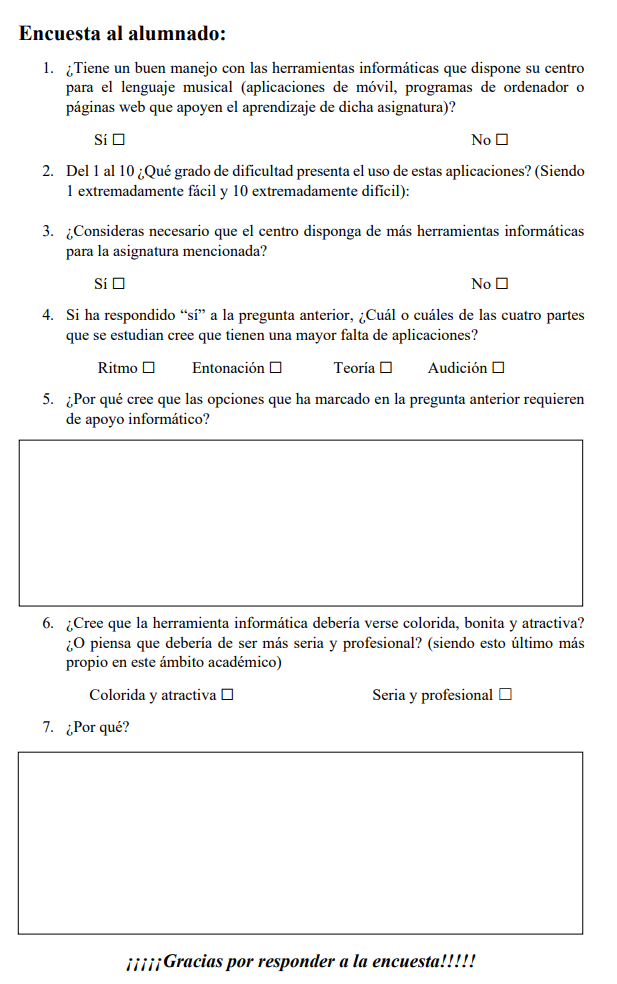
\includegraphics[width=0.45\linewidth]{Figuras/encuestaA.png}
    \caption{Encuesta al alumnado}
    \label{fig:enter-label}
\end{figure}

\newpage
Se exponen en una gráfica las respuestas a las preguntas 1, 3 y 6 en primer lugar, se debe tener en cuenta que el total de respuestas de cada pregunta de ambas gráficas varía un poco debido a que, en algunos casos, dicha respuesta estaba en blanco o no era adecuada:

\begin{figure}[h]
    \centering
    \subfloat[Respuestas de alumnado del conservatorio]{
    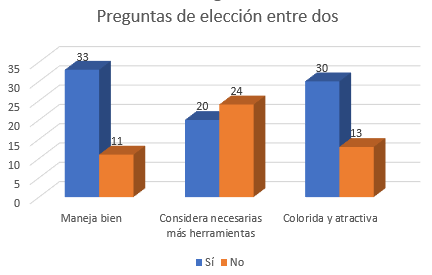
\includegraphics[width=0.5\linewidth]{Figuras/graficaSino.png}
    }
    \subfloat[Respuestas de alumnado de la escuela de música]{
        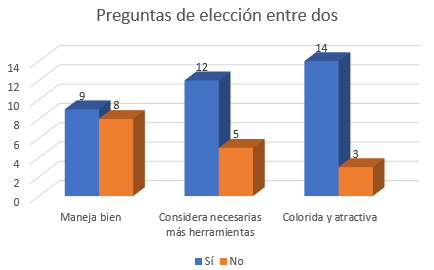
\includegraphics[width=0.5\linewidth]{Figuras/graficaSinoE.png}
    }
    \caption{Respuestas a las preguntas 1, 3 y 6}
    \label{fig:enter-label}
\end{figure}

Las respuestas de la pregunta 4 también han sido reflejadas en una gráfica:

\begin{figure}[h]
    \centering
    \subfloat[Respuestas de alumnado del conservatorio]{
    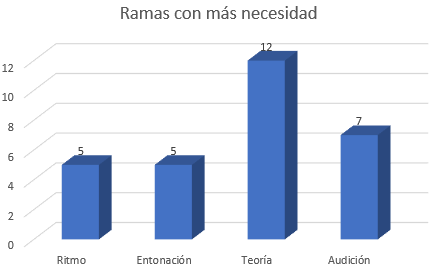
\includegraphics[width=0.5\linewidth]{Figuras/graficaRamasC.png}
    }
    \subfloat[Respuestas de alumnado de la escuela de música]{
        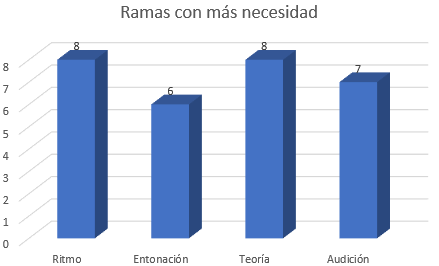
\includegraphics[width=0.5\linewidth]{Figuras/graficaRamasE.png}
    }
    \caption{Respuestas a las pregunta 4}
    \label{fig:enter-label}
\end{figure}

Cabe destacar que la media en la pregunta 2 ha sido de \textbf{4.68} para el conservatorio y de \textbf{2.58}.

Para las preguntas 5 y 7 se han seleccionado las mejores respuestas:

\begin{itemize}
\item Mejores respuestas de la pregunta 5:
\begin{itemize}
\item (Marcó todas las opciones en la pregunta 4) "Ninguna tiene apoyo informático y es necesario poder acceder al material desde casa".
\item (Marcó teoría en la pregunta 4) "Porque se debe poder acceder al contenido de clases anteriores para que no caiga en el olvido".
\item (Marcó teoría en la pregunta 4) "Porque en las calificaciones de las actividades de teoría actualmente no sé puede saber en qué te has equivocado".
\end{itemize}
\item Mejores respuestas de la pregunta 7:
\begin{itemize}
\item (Marcó ambas en la pregunta 6) "Creo que podría ser ambas cosas".
\item (Marcó colorida y atractiva en la pregunta 6) "Al llamar más la atención se crea un ambiente más llevadero y también es importante disfrutar un poco de nuestras responsabilidades".
\end{itemize}
\end{itemize}

Por lo tanto, se sacan las siguientes conclusiones:
\begin{enumerate}
\item En la escuela de música están mucho más de acuerdo en querer más herramientas informáticas y, a su vez, les cuesta menos el uso de las herramientas actuales, muy posiblemente sea debido a que en el conservatorio, el alumnado es generalmente mayor que en la escuela de música además de que, por experiencia personal, suele haber apuntados más adultos y es muy posible que estén menos dispuestos al uso de nuevos servicios.
\item Están bastante de acuerdo en que el software debe ser colorido y atractivo.
\item En contradicción con los profesores, creen más necesario reforzar los recursos informáticos dedicados a la teoría. También encuentran necesidad en la audición y el ritmo mientras que la entonación quedaría un peldaño por debajo.
\item Algunos aspectos referentes a la funcionalidad de software mencionados en las respuestas son la necesidad de poder acceder a material antiguo y desde casa y poder saber por qué se ha cometido un error en las correcciones de teoría. 
\end{enumerate}
\section {Herramientas actuales}

Ambos profesores se sirven de la aplicación web \textbf{EstudioMusica} y parece ser que las escuelas de música generalmente también usan herramientas incluidas con el material físico (libros de texto por ejemplo).
\newpage
\section {Necesidades detectadas}

Mezclando las necesidades de profesorado y alumnado, se llega a las siguientes conclusiones:

\begin{enumerate}
\item Es muy necesario apoyar a los centros de educación musical en cuanto a recursos informáticos debido a la escasez de las mismas.
\item En general, profesorado y alumnado está a favor de incentivar la informática en las aulas.
\item Es de vital importancia que las aplicaciones sean coloridas y atractivas.
\item Las ramas más importantes son la auditiva por parte del profesorado y la teórica por parte del alumnado. También se ha mencionado que podría ser muy útil reforzar la rama de la entonación en las etapas iniciales del estudio de la asignatura.
\item Es necesario crear una funcionalidad tipo cuestionario, en la cual, se puedan añadir las correcciones y justificación de por qué está bien o mal un ejercicio. También podría ser útil que el servicio fuera accesible desde casa y el material antiguo se mantuviera en el mismo. 
\end{enumerate}

\chapter {Estudio bibliográfico}
\section {Introducción}

El siguiente aspecto a tratar es la bibliografía. Una vez definidas unas conclusiones de la investigación previa, es necesario conocer qué documentación existe relacionada con el ámbito abarcado para  extraer y sintetizar una información de interés de cara a la construcción de la solución. Por lo tanto, es necesario establecer unos pasos a seguir que permitan obtener la documentación necesaria, de manera que, se ha elegido hacer uso de la MLR (Mapping Literature Review), ya que establece una metodología marcada propia del dominio de la informática.

Los pasos a seguir serán los siguientes:

\begin{enumerate}
\item Definición de la pregunta de interés y los criterios de inclusión y exclusión de los estudios.
\item Localización y selección de la documentación relevante.
\item Síntesis de la información de la selección.
\item Análisis e interpretación de los resultados presentados.
\end{enumerate}

\section {Mapping Literature Review}

\subsection{Definición la cadena de búsqueda y criterios}

En primer lugar, deben tener en cuenta los siguientes componentes clave:

\begin{itemize}
\item Población específica y contexto: Áreas de conocimiento del Software enfocado a la enseñanza del lenguaje musical.
\item Intervención: Funcionalidades y características interesantes desde el punto de vista pedagógico del lenguaje musical.
\item Comparación: Otros Software dedicados a la enseñanza del lenguaje musical
\item Resultado: Necesidades y conclusiones para una solución.
\end{itemize}
\newpage
Tras ello, se formulan una serie de preguntas en base a lo anterior:
\begin{enumerate}
\item ¿Que Software/s son más usados en la enseñanza del lenguaje musical?
\item ¿Que características debe tener un Software para que sea pedagógico desde el punto de vista musical?
\item ¿Que características son más importantes en un Software para la asignatura?
\item ¿Que necesidades no están cubiertas por el Software actual?
\end{enumerate}
Una vez identificadas las preguntas, es necesario crear una cadena de búsqueda que se encargue de encontrar documentación dedicada tan solo a responderlas. La cadena sería la siguiente:

("software" OR "system" OR "application" OR "service") AND ("musical language teaching" OR "musical language education" OR "musical language pedagogy") AND ("requirements" OR "charasteristics" OR "functionality")

Pero debido a que ninguna biblioteca daba resultados (excepto Google Scholar por ser muy genérica), se han tenido que disminuir en gran medida los términos de la cadena de búsqueda finalmente:

\textbf{("software" OR "system" OR "application" OR "service") AND ("pedagogy" OR "teaching") AND "musical language"}

Esto es consecuencia de que los temas tratados son muy dispares y es muy posible que exista muy poca documentación en la que se encuentren relacionados.

Por último, se han seleccionado los siguientes criterios de exclusión:

\begin{itemize}
\item No es accesible (documento privado o de pago).
\item No abarca cualquiera de los dos grandes temas (informática y/o lenguaje musical) y/o no los relaciona en ningún punto.
\item No está escrito en inglés o español.
\end{itemize}

\subsection{Selección de documentación relevante}
 Los motores de búsqueda utilizados han sido: Google Scholar, Scopus y Association for Computing Machinery (ACM) Library y UVAdoc, este último, porque al hacer búsquedas previas en crudo para analizar los campos, en la universidad de Valladolid (a la cual pertenece el repositorio mencionado), ya se habían hecho algunos TFGs similares. Para el motor de búsqueda de google se han analizado tan solo los primeros 50 resultados ya que, a partir de ahí, comenzaban a tener muy poca relevancia. 
 \newpage
 El flujograma ha sido el siguiente:
 
 \tikzstyle{block} = [rectangle, draw, node distance=4cm,
    text width=7em, text centered, rounded corners, minimum height=4em]
\tikzstyle{line} = [draw, -latex']
\tikzstyle{cloud} = [draw, ellipse, node distance=4cm,
    minimum height=1cm, text width=5.5em, text badly centered]
\begin{figure} [h]
\centering
\begin{tikzpicture}

    % Place nodes
    \node [block] (School) {Google Schoolar n=50};
    \node [block, right of=School] (Scopus) {Scopus n=4};
    \node [block, right of=Scopus] (ACM) {ACM Library n=15};
    \node [block, right of=ACM] (UVA) {UVAdoc n=5};
    \node [cloud, below] (docsEx) at (6, -3) {Documentación excluida tras aplicar los criterios y revisar duplicados n=69};
    \node [block, below] at (6, -10) (docs) {Documentación a revisar tras ser aplicados los criterios n=5};
    
    % Draw edges
    \path [line] (School) -- node {47}(docsEx);
    \path [line] (Scopus) -- node {4}(docsEx);
    \path [line] (ACM) -- node {15}(docsEx);
    \path [line] (UVA) -- node {3}(docsEx);
    \path [line] (docsEx) to[bend right] node {Scollar n = 3} (docs);
    \path [line] (docsEx) to[bend left] node {UVAdoc n=2} (docs);
     
    
\end{tikzpicture}
\caption{Flujograma de la Mapping Review}
\end{figure}
A pesar de la baja cantidad de documentos a revisar, abrir los términos de búsqueda para obtener más resultados no es una buena opción puesto que, el número de documentos irrelevantes ya es grande y solo se obtendrían aún más resultados innecesarios. Esto se debe a que, el marco teórico establecido que combina la informática con la música está bastante poco explorado aún.

\newpage

Esta es la documentación obtenida (ordenada de por fecha de publicación descendente):

\begin{table}[H]
\centering
\begin{tabularx}{\textwidth}{|l|l|l|X|X|}
\hline
\textbf{Fecha} 
& \multicolumn{4}{c|}{\textbf{Documentación recogida}} \\ \hline

\textbf{Datos} 
& \multicolumn{1}{|c|}{\textbf{Sitio de publicación}} & \multicolumn{1}{|c|}{\textbf{Tipo}} & \multicolumn{2}{>{\centering\arraybackslash}X|}{\textbf{Título}} \\ \hline

\multicolumn{1}{|c|}{2022} 
& \multicolumn{1}{c|}{UVAdoc} 
& \multicolumn{1}{c|}{Trabajo técnico} 
& \multicolumn{2}{>{\centering\arraybackslash}X|}{El lenguaje musical a través de las TIC en educación primaria} \\ \hline

\multicolumn{1}{|c|}{2018} 
& \multicolumn{1}{c|}{AtlantisPress} 
& \multicolumn{1}{c|}{Artículo} 
& \multicolumn{2}{>{\centering\arraybackslash}X|}{Music Computer Technologies and Interactive Systems of Education in Digital Age School} \\ \hline

\multicolumn{1}{|c|}{2017} 
& \multicolumn{1}{c|}{UVAdoc} 
& \multicolumn{1}{c|}{Trabajo técnico} 
& \multicolumn{2}{>{\centering\arraybackslash}X|}{Aplicación informática para la introducción del lenguaje musical (Leemusica) en dispositivos móviles} \\ \hline

\multicolumn{1}{|c|}{2015} 
& \multicolumn{1}{c|}{Hejmec Journal} 
& \multicolumn{1}{c|}{Artículo} 
& \multicolumn{2}{>{\centering\arraybackslash}X|}{Online Gaming to Learn Music and English Language in Music and Ballet School Solfeggio Education} \\ \hline

\multicolumn{1}{|c|}{2014} 
& \multicolumn{1}{c|}{Life Science Journal}  
& \multicolumn{1}{c|}{Artículo} 
& \multicolumn{2}{>{\centering\arraybackslash}X|}{Multimedia technologies as a tool for teaching supervision over the students' skills (within the course on “music theory training”)} \\ \hline

\end{tabularx}
\caption{Documentación recogida}
\end{table}



\subsection{Resultados obtenidos}

Como se ha descrito al principio de la revisión, el objetivo es encontrar soluciones o respuestas a una serie de problemáticas concretas que nos permitirán deducir una serie de conclusiones válidas para el proyecto. Para ello, se hará una breve síntesis de cada uno de los documentos enfocada en responder a las preguntas expuestas. 

\subsubsection{El lenguaje musical a través de las TIC en educación primaria}

Este primer documento es un Trabajo de Fin de Grado de la Universidad de Valladolid que consiste en la creación de un blog que funcione como apoyo para la enseñanza del lenguaje musical y, por tanto, se apoya mucho a su vez, en otro tipo de herramientas centrando su proyecto en la innovación, el ámbito pedagógico y el método de aprendizaje que deben seguir los alumnos sobre todo teniendo en cuenta que son en su mayoría de edades muy tempranas. Las herramientas en las que hace énfasis y en las se podría poner el foco son editores de partituras como Musescore o Noteflight, editores de audio como Audacity y aplicaciones de encuestas o juegos como Kahoot o Quizziz, por lo tanto, se deduce que las funcionalidades más interesantes que expone son las que aportan dichas herramientas. 
También, al tocar la parte de la innovación, insiste en el punto de que es contradictorio el hecho de que la asignatura sea impartida desde un punto de vista tan teórico, puesto que, es muy importante para el músico tener una formación práctica siendo esta, además, una vía mucho más amena, por lo tanto, es importante por la parte pedagógica que el alumno interaccione por su cuenta y tenga forma de trabajar los contenidos sin necesidad del estudio de memorización establecido actualmente. Por último, destaca que es importante llevar a cabo este proceso poco a poco, pues hay aún muchos profesores que están habituados a un sistema muy teórico y tradicional sin apoyarse demasiado en las TIC y que sería imposible realizar una adaptación de golpe, debido a ello, es importante encontrar un balance entre las innovaciones y el sistema actual.

\subsubsection{Music Computer Technologies and Interactive Systems of Education in Digital Age School}

En segundo lugar, se encuentra un artículo a modo de análisis de la influencia y presencia de la tecnología en el aprendizaje de la música así como sus ventajas e inconvenientes. Además, se comenta sobre un nuevo software llamado "Soft Way to Mozart System", el cual, trata de paliar esas necesidades que actualmente se presentan a la hora de aprender a tocar un instrumento. Al parecer, en este caso, trata más del aprendizaje del instrumento en sí que del lenguaje musical, aún así se nos aporta la información de que, mediante el software, existe una posibilidad muy grande de apoyar la enseñanza de la música en general. Además, cabe destacar, que una de las claves es que los alumnos, al ser de edades tempranas, es muy importante que puedan interactuar con las herramientas y no sea el profesor el único que lo haga.

\subsubsection{Aplicación informática para la introducción del lenguaje musical}

En el siguiente documento, se presenta otro Trabajo de Fin de Grado de la Universidad de Valladolid que consiste en el desarrollo de una aplicación para la enseñanza del lenguaje musical (más enfocado al desarrollo que el anterior) en edades tempranas como educación infantil. Vuelve a nombrar una serie de herramientas compatibles con el aprendizaje del asignatura como MuseScore, Audacity o creadores de encuestas/actividades e incluso algunas nuevas como Hydrogen que sirve para crear patrones de percusión con los que trabajar el ritmo con los alumnos y Band in a Box para patrones melódicos en este caso. 
En este caso, el objetivo de la herramienta es que los alumnos sean partícipes de la herramienta puesto que, para alumnos de educación infantil, los recursos creados hasta ahora los tiene que usar el profesor debido a su dificultad. Para ello, centra mucho su aplicación en la pedagogía a través del diseño, no solo haciéndolo llamativo, sino también usando colores para diferenciar notas entre otros recursos psicológicos. Por último, vuelve a hacerse énfasis en que la innovación no debe llegar de forma brusca, en este caso, debido a que la tecnología es un recurso complementario y no puede condicionar los contenidos que se dan en la asignatura, así como quitar demasiado tiempo al profesor para la enseñanza de los mismos. 

\subsubsection{Online Gaming to Learn Music and English Language in Music and Ballet School Solfeggio Education}

A continuación, se trata un artículo que se centra en el enriquecimiento que ganan los alumnos de música y otras artes en general al jugar videojuegos exponiendo que, a día de hoy, es muy importante desarrollar más recursos TIC enfocados en la música. El documento aporta una serie de páginas web con juegos on-line musicales que se pueden usar como software de referencia, estas son "Classics for Kids Games" y "New York Philharmonic Kidzone".

\subsubsection{Multimedia technologies as a tool for teaching supervision over the students' skills (within the course on “music theory training”)}
Por último, se revisa este artículo que consiste en la búsqueda de métodos para poder evaluar las habilidades del alumno de música, y parece ser que el mejor para ello es las tecnologías multimedia. También incide en las competencias a evaluar y la metodología. Para el proyecto actual, tan solo es importante tomar en cuenta lo mencionado al principio sobre que es muy importante establecer la posibilidad de que se pueda llevar una supervisión y evaluación del alumno mediante los recursos TIC.

\subsection{Conclusiones}

Tras analizar los diferentes documentos se sacan las siguientes conclusiones:

\begin{enumerate}
\item Los software que se recomiendan, en general, son herramientas de apoyo que no pueden abarcar el grueso del temario de la asignatura y, además, son recursos muy completos que no pueden ser introducidos en este trabajo ya que por sí solos son un proyecto muy completo (línea de trabajo futura), exceptuando los juegos y cuestionarios en los que sí podría ser interesante poner el foco.
\item Se insiste mucho en la pedagogía en todos los documentos ya que la asignatura es impartida a personas de edades muy tempranas (desde 8 a 14 años generalmente), de hecho, no es importante tan solo crear un diseño llamativo sino que también la propia discriminación de colores u otras funcionalidades del tipo pueden ayudar a obtener una serie de enseñanzas concretas al alumnado, además de ayudar a personas con distintos tipos de problemas visuales u otras patologías y, sobre todo, que sea sencillo de usar para que pueda interactuar el alumnado y para que pueda ser gestionada por el profesorado sin demasiada formación en las TIC .
\item Las características señaladas, por tanto, podrían ser, el desarrollo de cuestionarios, atender al diseño responsive, usabilidad y seguimiento y evaluación del alumnado.
\item Actualmente, el principal problema de las herramientas no es la falta de funcionalidades, sino el hecho de que no pueden abarcar la asignatura por sí solas, por tanto, es necesario aunar las funcionalidades más básicas para la asignatura en una sola herramienta que, además, permita establecer un sistema de evaluación para que pueda ser el epicentro de la enseñanza de la asignatura que, además, sea fácil de manejar por todo tipo de usuarios.
\end{enumerate}

\chapter {Definición del problema a resolver}
La investigación y el estudio bibliográfico han dejado definidas una serie de necesidades que deben ser cubiertas por la solución a desarrollar pero con un nivel de abstracción muy alto, por tanto, se debe transformar la información a un nivel más objetivo.
Para ello, se creará, en primer lugar, una especificación formal donde se redactarán todos los aspectos de la aplicación de una forma mucho más metódica y se establecerán unos objetivos funcionales resumidos, combinando así el lenguaje natural en el que se encuentra la información obtenida previamente con la objetividad a la que se desea llegar en el siguiente paso.
Posteriormente, esta información se plasmará en un diagrama de casos de uso del sistema que permita entender de una forma más visual y esquemática el funcionamiento de la aplicación y se describirán en detalle cada uno de los actores y casos de uso, junto con sus requisitos funcionales asociados, incluyendo la secuencia de pasos que garantizan su correcto cumplimiento, además se abordarán los requisitos no funcionales que condicionan la calidad y comportamiento esperado del sistema.
Por último, se definirán las tecnologías a utilizar y la arquitectura de la solución para tener una visión global de la solución a desarrollar antes de comenzar con el desarrollo de la misma.
\section{Especificación formal de la solución}

El sistema permitirá el acceso mediante un mecanismo de inicio de sesión en el que podrán autenticarse tres tipos de usuarios: administrador, profesor y alumno. Cada usuario tendrá acceso únicamente a las funcionalidades correspondientes a su rol, sin posibilidad de utilizar las funciones asignadas a otros.

No existirá un proceso de registro automático. El administrador será creado de forma manual y, una vez dentro de la aplicación, tendrá la capacidad de crear las cuentas de los profesores. Para ello, deberá introducir los siguientes datos: nombre, primer apellido, segundo apellido y dirección de correo electrónico. Se realizará una comprobación de validez de los datos introducidos (formato correcto del nombre, de los apellidos y del correo electrónico) y una verificación de unicidad del correo electrónico en la base de datos.

En el proceso de creación, el sistema generará automáticamente un nombre de usuario a partir de la primera letra del nombre y de los apellidos. Por ejemplo, para un usuario denominado José Luis Garrido Castro, el identificador generado será jgc. En caso de que existan coincidencias con identificadores ya presentes en la base de datos, se añadirá un número consecutivo equivalente al total de usuarios con la misma raíz más uno, de modo que si ya existen 40 usuarios con identificadores iniciados en jgc, el nuevo identificador será jgc41. La contraseña será generada automáticamente mediante el uso de un servicio externo de generación de contraseñas seguras. Una vez creadas las credenciales, estas serán enviadas por correo electrónico al profesor.

El profesor, a su vez, tendrá la capacidad de crear cuentas de alumnos mediante un procedimiento equivalente al descrito para la creación de profesores.

Además, el profesor podrá crear grupos de clase, añadir alumnos a los mismos, eliminarlos o eliminar grupos completos. Un alumno podrá pertenecer a varios grupos de forma simultánea.

También podrá enviar mensajes a unos alumnos o cursos completos determinados y otra ventana donde podrá adjuntar las calificaciones generales del curso seleccionando a un alumno en concreto.

El sistema dispondrá de un área denominada administración en la que estarán disponibles las operaciones mencionadas anteriormente.

Fuera de esta sección, la aplicación contará con cuatro apartados denominados \textbf{Ritmo, Entonación, Audición y Teoría}. Cada apartado estará compuesto por dos secciones diferenciadas:
\begin{enumerate}
\item \textbf{Libro del curso}: permitirá al profesor subir un único archivo en formato PDF correspondiente al curso seleccionado. Si se sube un nuevo archivo, el anterior será sustituido. El profesor podrá eliminar o reemplazar el archivo en cualquier momento.

\item \textbf{Tareas a realizar}: permitirá al profesor crear tareas asociadas a un curso determinado. Cada tarea constará de una descripción y, opcionalmente, de un material de apoyo en formato PDF, MP3 o MP4. También se definirá una fecha límite de entrega. Las tareas podrán calificarse individualmente, modificarse y/o eliminarse en cualquier momento, pero no se eliminarán automáticamente al llegar la fecha de entrega; se mantendrán hasta la finalización del curso. En el apartado de Teoría, las tareas podrán sustituirse (o no) por un cuestionario tipo test. Dicho cuestionario permitirá la creación de preguntas con opciones de respuesta, y cada pregunta podrá ir acompañada de un archivo en formato MP3.
\end{enumerate}
Los alumnos dispondrán de un área específica de notificaciones. En ella recibirán avisos cuando sean añadidos o eliminados de un curso o grupo, cuando se cree una nueva tarea, cuando se suba un libro del curso, cuando reciban una calificación (notificaciones del sistema) o un mensaje (notificaciones del profesor). Las notificaciones serán interactivas, permitiendo acceder directamente al recurso correspondiente.

Asimismo, los alumnos podrán acceder a los mismos cuatro apartados (Ritmo, Entonación, Audición y Teoría). En cada apartado se mostrarán las mismas dos secciones:
\begin{itemize}
\item En la sección Libro del curso, los alumnos podrán visualizar el archivo PDF correspondiente y descargarlo, pero no modificarlo.

\item En la sección Tareas a realizar, los alumnos podrán consultar la lista de tareas disponibles y realizar las entregas correspondientes. Los formatos permitidos serán PDF, MP3 o MP4, y/o bien un comentario textual dentro de la propia aplicación. En el caso de cuestionarios, el alumno accederá a una ventana específica donde podrá completarlo. El cuestionario no se considerará entregado hasta que el alumno pulse expresamente el botón de envío.
\end{itemize}
\section{Objetivos funcionales del sistema}
El objetivo principal del sistema es facilitar y mejorar la enseñanza del lenguaje musical mediante una plataforma que proporcione funcionalidades específicas tanto para profesores como para alumnos. Estos objetivos funcionales guían el desarrollo del sistema y aseguran que las necesidades pedagógicas y administrativas se cubran de forma eficiente y adaptada a las diferentes ramas del aprendizaje musical.
Los objetivos funcionales que se persiguen son los siguientes:

\begin{itemize}
  \item Permitir al profesorado crear, gestionar y visualizar grupos de alumnos, facilitando la organización y seguimiento académico.
  \item Gestionar el contenido educativo estructurado según las ramas del lenguaje musical: teoría, entonación, ritmo y audición.
  \item Proporcionar herramientas para que el profesor pueda crear, modificar, cerrar y eliminar tareas y cuestionarios específicos para cada rama.
  \item Facilitar la interacción del alumnado con las tareas y cuestionarios, incluyendo la entrega de trabajos y la realización de pruebas con autocorrección cuando corresponda.
  \item Permitir al profesorado revisar, calificar y gestionar las entregas y calificaciones de los alumnos de forma clara y accesible.
  \item Implementar un sistema de mensajería interna que facilite la comunicación entre profesores y alumnos, con notificaciones automáticas vinculadas a eventos relevantes.
  \item Permitir la gestión del material didáctico asociado a cada rama del aprendizaje musical, con capacidad de adaptación y personalización según las necesidades específicas de cada grupo de alumnos.
\end{itemize}

Estos objetivos funcionales proporcionan un marco claro para la posterior definición de los casos de uso y requisitos funcionales, asegurando que el sistema responda adecuadamente a las necesidades del entorno educativo para el que está diseñado.

\section {Diagrama UML de casos de uso del sistema}
Una vez definida la solución mediante lenguaje natural, se da el siguiente paso hacia el modelado de casos de uso.
\begin{figure}[H]
    \centering
    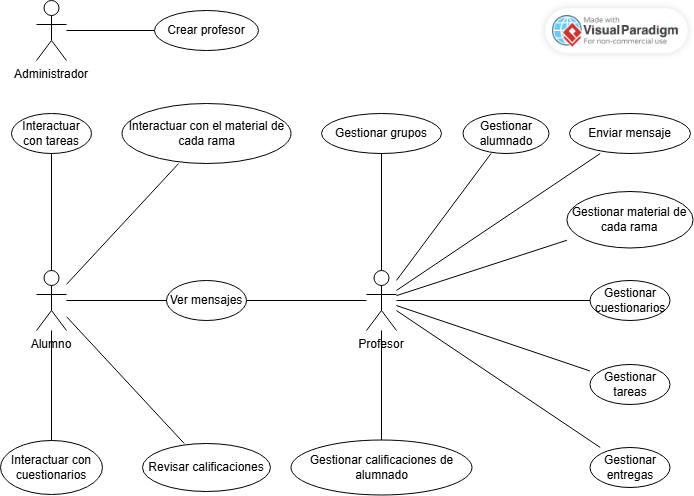
\includegraphics[width=1\linewidth]{Figuras/DCU.png}
    \caption{Diagrama UML de casos de uso del sistema}
\end{figure}
\section {Definición del diagrama de casos de uso}
El diagrama de casos de uso aporta una visión muy genérica y poco detallada y, aunque es mucho más objetiva que el lenguaje natural, se encuentra en un nivel de abstracción muy alto, por lo tanto, es necesario entrar en más detalle para cada uno de los elementos del diagrama.
\subsection {Actores}
Se pueden observar cuatro actores principales, cada uno con su respectivo rol:
\begin{table}[h!]
\centering
\begin{tabularx}{\textwidth}{
  |>{\centering\arraybackslash}l
  |>{\centering\arraybackslash}X|
}
\hline
\textbf{ID del actor} & \textbf{ACT-1} \\ \hline
\textbf{Nombre del actor} & Usuario no autenticado \\ \hline
\textbf{Rol} & Usuario que accede al sistema con el único objetivo de iniciar sesión. \\ \hline
\end{tabularx}
\caption{Actor 1}
\end{table}
\begin{table}[h!]
\centering
\begin{tabularx}{\textwidth}{
  |>{\centering\arraybackslash}l
  |>{\centering\arraybackslash}X|    
}
\hline
\textbf{ID del actor} & \textbf{ACT-2} \\ \hline
\textbf{Nombre del actor} & Administrador \\ \hline
\textbf{Rol} & Usuario autenticado con el objetivo de crear a los usuarios con rol de profesor en el sistema. \\ \hline
\end{tabularx}
\caption{Actor 2}
\end{table}
\begin{table}[h!]
\centering
\begin{tabularx}{\textwidth}{
  |>{\centering\arraybackslash}l
  |>{\centering\arraybackslash}X|
}
\hline
\textbf{ID del actor} & \textbf{ACT-3} \\ \hline
\textbf{Nombre del actor} & Profesor \\ \hline
\textbf{Rol} & Usuario autenticado con el objetivo de crear usuarios con el rol alumno y gestionar el contenido académico dirigido a los mismos en el sistema. \\ \hline
\end{tabularx}
\caption{Actor 3}
\end{table}
\begin{table}[h!]
\centering
\begin{tabularx}{\textwidth}{
  |>{\centering\arraybackslash}l
  |>{\centering\arraybackslash}X|
}
\hline
\textbf{ID del actor} & \textbf{ACT-4} \\ \hline
\textbf{Nombre del actor} & Alumno \\ \hline
\textbf{Rol} & Usuario autenticado con el objetivo de acceder al contenido e interactuar con el mismo a través del sistema. \\ \hline
\end{tabularx}
\caption{Actor 4}
\end{table}
\subsection {Casos de uso}
Para definir los casos de uso del sistema la mejor forma de hacerlo es, como en cualquier otro proyecto de desarrollo de software, mediante los requisitos funcionales que lo conforman.
\subsubsection {Definición general}
\begin{table}[H]
\centering
\begin{tabularx}{\textwidth}{
  |>{\centering\arraybackslash}l
  |>{\centering\arraybackslash}X|}
\hline
\textbf{Nombre} & {\textbf{Iniciar sesión}} \\ \hline

\textbf{Descripción} & Permitir al usuario no autenticado iniciar sesión en el sistema proporcionando sus credenciales y, en caso de éxito, tendrá acceso a las funcionalidades del actor que tenga asignado en el sistema. \\ \hline
\textbf{Actor} & ACT-1 \\ \hline
\textbf{Requisitos funcionales} & RF-01 \\ \hline
\end{tabularx}
\caption{Caso de uso: Iniciar sesión}
\end{table}
\begin{table}[H]
\centering
\begin{tabularx}{\textwidth}{
  |>{\centering\arraybackslash}l
  |>{\centering\arraybackslash}X|}
\hline
\textbf{Nombre} & {\textbf{Recuperar contraseña}} \\ \hline

\textbf{Descripción} & Permitir al usuario recuperar el acceso a su cuenta mediante la verificación de su dirección de correo. \\ \hline
\textbf{Actor} & ACT-1 \\ \hline
\textbf{Requisitos funcionales} & RF-02 \\ \hline
\end{tabularx}
\caption{Caso de uso: Recuperar contraseña}
\end{table}

\begin{table}[H]
\centering
\begin{tabularx}{\textwidth}{
  |>{\centering\arraybackslash}l
  |>{\centering\arraybackslash}X|}
\hline
\textbf{Nombre} & {\textbf{Crear profesor}} \\ \hline

\textbf{Descripción} & Permitir al administrador crear nuevos usuarios con rol de profesor en el sistema, proporcionando los datos necesarios y validando la información. \\ \hline
\textbf{Actor} & ACT-2 \\ \hline
\textbf{Requisitos funcionales} & RF-03 \\ \hline
\end{tabularx}
\caption{Caso de uso: Crear profesor}
\end{table}
\begin{table}[H]
\centering
\begin{tabularx}{\textwidth}{
  |>{\centering\arraybackslash}l
  |>{\centering\arraybackslash}X|}
\hline
\textbf{Nombre} & {\textbf{Crear alumno}} \\ \hline

\textbf{Descripción} & Permitir al profesor crear nuevos usuarios con rol de alumno en el sistema, proporcionando los datos necesarios y validando la información. \\ \hline
\textbf{Actor} & ACT-3 \\ \hline
\textbf{Requisitos funcionales} & RF-05 RF-04 \\ \hline
\end{tabularx}
\caption{Caso de uso: Crear alumno}
\end{table}
\begin{table}[H]
\centering
\begin{tabularx}{\textwidth}{
  |>{\centering\arraybackslash}l
  |>{\centering\arraybackslash}X|}
\hline
\textbf{Nombre} & {\textbf{Gestionar grupos}} \\ \hline
\textbf{Descripción} & Permitir al profesor crear nuevos grupos, revisar los que ha creado y elegir un grupo para trabajar con él. \\ \hline
\textbf{Actor} & ACT-3\\ \hline
\textbf{Requisitos funcionales} & RF-06 RF-07 RF-08 \\ \hline
\end{tabularx}
\caption{Caso de uso: Gestionar grupos}
\end{table}
\begin{table}[H]
\centering
\begin{tabularx}{\textwidth}{
  |>{\centering\arraybackslash}l
  |>{\centering\arraybackslash}X|}
\hline
\textbf{Nombre} & {\textbf{Enviar mensaje}} \\ \hline

\textbf{Descripción} & Permitir al profesor enviar mensajes a los alumnos de un grupo seleccionado. \\ \hline
\textbf{Actor} & ACT-3\\ \hline
\textbf{Requisitos funcionales} & RF-09 \\ \hline
\end{tabularx}
\caption{Caso de uso: Enviar mensaje}
\end{table}
\begin{table}[H]
\centering
\begin{tabularx}{\textwidth}{
  |>{\centering\arraybackslash}l
  |>{\centering\arraybackslash}X|}
\hline
\textbf{Nombre} & {\textbf{Gestionar material de cada rama}} \\ \hline

\textbf{Descripción} & Permitir al profesor gestionar el material de cada rama de la asignatura. \\ \hline
\textbf{Actor} & ACT-3\\ \hline
\textbf{Requisitos funcionales} & RF-10 RF-11 RF-12 \\ \hline
\end{tabularx}
\caption{Caso de uso: Gestionar material de cada rama}
\end{table}
\begin{table}[H]
\centering
\begin{tabularx}{\textwidth}{
  |>{\centering\arraybackslash}l
  |>{\centering\arraybackslash}X|}
\hline
\textbf{Nombre} & {\textbf{Gestionar tareas}} \\ \hline

\textbf{Descripción} & Permitir al profesor gestionar las tareas de cada rama de la asignatura. \\ \hline
\textbf{Actor} & ACT-3\\ \hline
\textbf{Requisitos funcionales} & RF-13 RF-14 RF-15 RF-16 RF-17 \\ \hline
\end{tabularx}
\caption{Caso de uso: Gestionar tareas}
\end{table}
\begin{table}[H]
\centering
\begin{tabularx}{\textwidth}{
  |>{\centering\arraybackslash}l
  |>{\centering\arraybackslash}X|}
\hline
\textbf{Nombre} & {\textbf{Gestionar cuestionarios}} \\ \hline

\textbf{Descripción} & Permitir al profesor gestionar los cuestionarios de la rama de teoría de la asignatura. \\ \hline
\textbf{Actor} & ACT-3\\ \hline
\textbf{Requisitos funcionales} & RF-18 RF-19 RF-20 RF-21 RF-22 \\ \hline
\end{tabularx}
\caption{Caso de uso: Gestionar entregas}
\end{table}
\begin{table}[H]
\centering
\begin{tabularx}{\textwidth}{
  |>{\centering\arraybackslash}l
  |>{\centering\arraybackslash}X|}
\hline
\textbf{Nombre} & {\textbf{Gestionar entregas}} \\ \hline

\textbf{Descripción} & Permitir al profesor gestionar las entregas de las tareas de los alumnos. \\ \hline
\textbf{Actor} & ACT-3\\ \hline
\textbf{Requisitos funcionales} & RF-23 RF-24 RF-25\\ \hline
\end{tabularx}
\caption{Caso de uso: Gestionar entregas}
\end{table}
\begin{table}[H]
\centering
\begin{tabularx}{\textwidth}{
  |>{\centering\arraybackslash}l
  |>{\centering\arraybackslash}X|}
\hline
\textbf{Nombre} & {\textbf{Gestionar calificaciones del alumnado}} \\ \hline

\textbf{Descripción} & Permitir al profesor gestionar las calificaciones generales del curso de los alumnos. \\ \hline
\textbf{Actor} & ACT-3\\ \hline
\textbf{Requisitos funcionales} & RF-26 RF-27\\ \hline
\end{tabularx}
\caption{Caso de uso: Gestionar calificaciones del alumnado}
\end{table}
\begin{table}[H]
\centering
\begin{tabularx}{\textwidth}{
  |>{\centering\arraybackslash}l
  |>{\centering\arraybackslash}X|}
\hline
\textbf{Nombre} & {\textbf{Ver mensajes}} \\ \hline

\textbf{Descripción} & Permitir al alumno y al profesor ver los mensajes. \\ \hline
\textbf{Actor} & ACT-3 ACT-4\\ \hline
\textbf{Requisitos funcionales} & RF-28\\ \hline
\end{tabularx}
\caption{Caso de uso: Ver mensajes}
\end{table}
\begin{table}[H]
\centering
\begin{tabularx}{\textwidth}{
  |>{\centering\arraybackslash}l
  |>{\centering\arraybackslash}X|}
\hline
\textbf{Nombre} & {\textbf{Interactuar con el material de cada rama}} \\ \hline

\textbf{Descripción} & Permitir al alumno interactuar con el material de cada rama. \\ \hline
\textbf{Actor} & ACT-4\\ \hline
\textbf{Requisitos funcionales} & RF-10\\ \hline
\end{tabularx}
\caption{Caso de uso: Interactuar con el material de cada rama}
\end{table}
\begin{table}[H]
\centering
\begin{tabularx}{\textwidth}{
  |>{\centering\arraybackslash}l
  |>{\centering\arraybackslash}X|}
\hline
\textbf{Nombre} & {\textbf{Revisar calificaciones}} \\ \hline

\textbf{Descripción} & Permitir al alumno revisar las calificaciones. \\ \hline
\textbf{Actor} & ACT-4\\ \hline
\textbf{Requisitos funcionales} & RF-25\\ \hline
\end{tabularx}
\caption{Caso de uso: Revisar calificaciones}
\end{table}
\begin{table}[H]
\centering
\begin{tabularx}{\textwidth}{
  |>{\centering\arraybackslash}l
  |>{\centering\arraybackslash}X|}
\hline
\textbf{Nombre} & {\textbf{Interactuar con tareas}} \\ \hline

\textbf{Descripción} & Permitir al alumno interactuar con las tareas. \\ \hline
\textbf{Actor} & ACT-4\\ \hline
\textbf{Requisitos funcionales} & RF-13 RF-29\\ \hline
\end{tabularx}
\caption{Caso de uso: Interactuar con tareas}
\end{table}
\begin{table}[H]
\centering
\begin{tabularx}{\textwidth}{
  |>{\centering\arraybackslash}l
  |>{\centering\arraybackslash}X|}
\hline
\textbf{Nombre} & {\textbf{Interactuar con cuestionarios}} \\ \hline

\textbf{Descripción} & Permitir al alumno interactuar con los cuestionarios. \\ \hline
\textbf{Actor} & ACT-4\\ \hline
\textbf{Requisitos funcionales} & RF-18 RF-30\\ \hline
\end{tabularx}
\caption{Caso de uso: Interactuar con cuestionarios}
\end{table}
\subsubsection {Requisitos funcionales}
\begin{table}[H]
\centering
\begin{tabularx}{\textwidth}{
  |>{\centering\arraybackslash}l
  |>{\centering\arraybackslash}X|}
\hline

\textbf{RF-01} & \textbf{Iniciar sesión} \\ \hline

\textbf{Descripción} & Permitir al usuario no autenticado iniciar sesión en el sistema proporcionando sus credenciales y, en caso de éxito, tendrá acceso a las funcionalidades del actor que tenga asignado en el sistema. \\ \hline

\textbf{Precondición} & El usuario no debe estar autenticado en el sistema. \\ \hline

\textbf{Secuencia de pasos} & 
\begin{enumerate}
  \item El usuario accede a la pantalla de inicio de sesión.
  \item El usuario introduce su nombre de usuario y contraseña.
  \item El sistema valida las credenciales introducidas.
  \item Si las credenciales son correctas, el sistema autentica al usuario.
  \item El sistema asigna al usuario el rol correspondiente y concede acceso a las funcionalidades habilitadas.
  \item El usuario es redirigido a la página principal o panel correspondiente a su rol.
\end{enumerate} \\ \hline

\textbf{Postcondición} & El usuario queda autenticado en el sistema con acceso a las funcionalidades correspondientes a su rol. \\ \hline

\textbf{Excepciones} & 
\begin{itemize}
  \item El usuario introduce credenciales incorrectas.
  \item Problemas de conexión con la base de datos.
\end{itemize} \\ \hline
\end{tabularx}
\caption{Requisito funcional: RF-01 Iniciar sesión}
\end{table}
\begin{table}[H]
\centering
\begin{tabularx}{\textwidth}{
  |>{\centering\arraybackslash}l
  |>{\centering\arraybackslash}X|}
\hline

\textbf{RF-02} & \textbf{Recuperar contraseña} \\ \hline

\textbf{Descripción} & Permitir al usuario recuperar el acceso a su cuenta mediante la verificación de su dirección de correo. \\ \hline

\textbf{Precondición} & El usuario debe tener acceso al correo electrónico asociado a su cuenta y no estar autenticado en el sistema. \\ \hline

\textbf{Secuencia de pasos} & 
\begin{enumerate}
  \item El usuario accede a la opción "Recuperar contraseña" desde la pantalla de inicio de sesión.
  \item El usuario introduce su dirección de correo electrónico registrada.
  \item El sistema verifica que el correo electrónico existe en la base de datos.
  \item El sistema actualiza la contraseña.
  \item El sistema envía la contraseña por correo y notifica al usuario del éxito.
\end{enumerate} \\ \hline

\textbf{Postcondición} & El usuario puede iniciar sesión con la nueva contraseña establecida. \\ \hline

\textbf{Excepciones} & 
\begin{itemize}
  \item El correo electrónico proporcionado no está registrado en el sistema.
  \item El sistema no puede conectarse a la base de datos o servicio de correo.
\end{itemize} \\ \hline
\end{tabularx}
\caption{Requisito funcional: RF-02 Recuperar contraseña}
\end{table}
\begin{table}[H]
\centering
\begin{tabularx}{\textwidth}{
  |>{\centering\arraybackslash}l
  |>{\centering\arraybackslash}X|}
\hline
\textbf{RF-03} & \textbf{Crear profesor} \\ \hline

\textbf{Descripción} & Permitir al administrador crear nuevos usuarios con rol de profesor en el sistema, proporcionando los datos necesarios. \\ \hline

\textbf{Precondición} & El administrador debe estar autenticado en el sistema. \\ \hline

\textbf{Secuencia de pasos} & 
\begin{enumerate}
  \item El administrador introduce los datos requeridos del profesor (nombre, apellidos y correo).
  \item El sistema valida los datos mediante RF-04.
  \item El sistema guarda el nuevo profesor.
  \item El sistema notifica al administrador que el profesor ha sido creado correctamente.
\end{enumerate} \\ \hline

\textbf{Postcondición} & El nuevo profesor queda registrado en el sistema y puede iniciar sesión con las credenciales asignadas. \\ \hline

\textbf{Excepciones} & 
\begin{itemize}
  \item Datos incompletos o inválidos introducidos por el administrador.
  \item Problemas de conexión con la base de datos.
\end{itemize} \\ \hline
\end{tabularx}
\caption{Requisito funcional: RF-03 Crear profesor}
\end{table}

\begin{table}[H]
\centering
\begin{tabularx}{\textwidth}{
  |>{\centering\arraybackslash}l
  |>{\centering\arraybackslash}X|}
\hline
\textbf{RF-04} & \textbf{Validación y generación automática de credenciales} \\ \hline

\textbf{Descripción} & Validar la información de creación de un nuevo usuario comprobando la unicidad del correo, formatos específicos para nombre, apellidos y correo, y generar automáticamente el username y la contraseña. \\ \hline

\textbf{Precondición} & Se reciben datos completos del profesor para validar y generar credenciales. \\ \hline

\textbf{Secuencia de pasos} & 
\begin{enumerate}
  \item El sistema comprueba que el correo no está registrado.
  \item El sistema valida que el correo tenga formato tipo ejemplo@ejemplo.com.
  \item El sistema valida que el nombre y apellidos solo contengan letras sin espacios ni caracteres inválidos.
  \item El sistema genera el username a partir de las siglas de nombre y apellidos.
  \item Si el username generado ya existe, se añade un identificador numérico para diferenciarlo.
  \item El sistema solicita a una API externa la generación de una contraseña segura.
  \item El sistema asocia el username y contraseña generados a la cuenta del profesor.
\end{enumerate} \\ \hline

\textbf{Postcondición} & Se dispone de credenciales únicas y válidas para el nuevo profesor, listas para su uso en el sistema. \\ \hline

\textbf{Excepciones} & 
\begin{itemize}
  \item El correo proporcionado ya está registrado.
  \item Los datos no cumplen con el formato requerido.
  \item Fallo en la comunicación con la API externa para generación de contraseña.
  \item Problemas técnicos al generar o asignar las credenciales.
\end{itemize} \\ \hline
\end{tabularx}
\caption{Requisito funcional: RF-04 Validación y generación automática de credenciales}
\end{table}
\begin{table}[H]
\centering
\begin{tabularx}{\textwidth}{
  |>{\centering\arraybackslash}l
  |>{\centering\arraybackslash}X|}
\hline
\textbf{RF-05} & \textbf{Crear alumno} \\ \hline

\textbf{Descripción} & Permitir al profesor crear nuevos usuarios con rol de alumno en el sistema, proporcionando los datos necesarios. \\ \hline

\textbf{Precondición} & El profesor debe estar autenticado en el sistema. \\ \hline

\textbf{Secuencia de pasos} & 
\begin{enumerate}
  \item El profesor introduce los datos requeridos del alumno (nombre, apellidos y correo).
  \item El sistema valida los datos mediante RF-04.
  \item El sistema guarda el nuevo alumno.
  \item El sistema notifica al profesor que el alumno ha sido creado correctamente.
\end{enumerate} \\ \hline

\textbf{Postcondición} & El nuevo alumno queda registrado en el sistema y puede iniciar sesión con las credenciales asignadas. \\ \hline

\textbf{Excepciones} & 
\begin{itemize}
  \item Datos incompletos o inválidos introducidos por el profesor.
  \item Problemas de conexión con la base de datos.
\end{itemize} \\ \hline
\end{tabularx}
\caption{Requisito funcional: RF-05 Crear alumno}
\end{table}
\begin{table}[H]
\centering
\begin{tabularx}{\textwidth}{
  |>{\centering\arraybackslash}l
  |>{\centering\arraybackslash}X|}
\hline
\textbf{RF-06} & \textbf{Crear grupo} \\ \hline

\textbf{Descripción} & Permitir al profesor crear nuevos grupos proporcionando la información necesaria (nombre del grupo y alumnos). \\ \hline

\textbf{Precondición} & El profesor debe estar autenticado en el sistema y tener usuarios creados \\ \hline

\textbf{Secuencia de pasos} & 
\begin{enumerate}
  \item El profesor accede a la sección de administración.
  \item El profesor introduce los datos requeridos para el grupo.
  \item El sistema valida la información introducida.
  \item El sistema guarda el nuevo grupo.
  \item El sistema crea las ramas de la asignatura vacías (sin ningún material aún) y las guarda.
  \item El sistema notifica al profesor que el grupo ha sido creado correctamente.
\end{enumerate} \\ \hline

\textbf{Postcondición} & El grupo queda registrado en el sistema asociado al profesor y los alumnos incluidos. \\ \hline

\textbf{Excepciones} & 
\begin{itemize}
  \item Datos inválidos introducidos por el profesor.
  \item Problemas de conexión con la base de datos.
\end{itemize} \\ \hline
\end{tabularx}
\caption{Requisito funcional: RF-06 Crear grupo}
\end{table}


\begin{table}[H]
\centering
\begin{tabularx}{\textwidth}{
  |>{\centering\arraybackslash}l
  |>{\centering\arraybackslash}X|}
\hline
\textbf{RF-07} & \textbf{Revisar grupos} \\ \hline

\textbf{Descripción} & Permitir al profesor visualizar la lista de grupos que ha creado previamente. \\ \hline

\textbf{Precondición} & El profesor debe estar autenticado en el sistema y tener grupos creados. \\ \hline

\textbf{Secuencia de pasos} & 
\begin{enumerate}
  \item El profesor accede a la sección de grupos.
  \item El sistema recupera y muestra la lista de grupos asociados al profesor.
  \item El profesor revisa los grupos mostrados.
\end{enumerate} \\ \hline

\textbf{Postcondición} & El profesor puede ver y seleccionar cualquier grupo de su lista para gestionar. \\ \hline

\textbf{Excepciones} & 
\begin{itemize}
  \item No existen grupos creados por el profesor.
  \item Problemas de conexión con la base de datos.
\end{itemize} \\ \hline
\end{tabularx}
\caption{Requisito funcional: RF-07 Listar grupos}
\end{table}


\begin{table}[H]
\centering
\begin{tabularx}{\textwidth}{
  |>{\centering\arraybackslash}l
  |>{\centering\arraybackslash}X|}
\hline
\textbf{RF-08} & \textbf{Seleccionar grupo} \\ \hline

\textbf{Descripción} & Permitir al profesor seleccionar un grupo creado para realizar acciones específicas o trabajar con su contenido. \\ \hline

\textbf{Precondición} & El profesor debe estar autenticado y haber creado al menos un grupo. \\ \hline

\textbf{Secuencia de pasos} & 
\begin{enumerate}
  \item El profesor visualiza la lista de grupos creados mediante RF-06.
  \item El profesor selecciona un grupo de la lista.
  \item El sistema carga los datos y funcionalidades correspondientes al grupo seleccionado.
  \item El profesor puede comenzar a trabajar con el grupo.
\end{enumerate} \\ \hline

\textbf{Postcondición} & El sistema queda configurado para trabajar con el grupo seleccionado. \\ \hline

\textbf{Excepciones} & 
\begin{itemize}
  \item El grupo seleccionado no existe.
  \item Problemas de carga o acceso a los datos del grupo.
\end{itemize} \\ \hline
\end{tabularx}
\caption{Requisito funcional: RF-08 Seleccionar grupo}
\end{table}
\begin{table}[H]
\centering
\begin{tabularx}{\textwidth}{
  |>{\centering\arraybackslash}l
  |>{\centering\arraybackslash}X|}
\hline
\textbf{RF-09} & \textbf{Enviar mensaje} \\ \hline

\textbf{Descripción} & Permitir al profesor enviar mensajes a los alumnos de un grupo seleccionado. \\ \hline

\textbf{Precondición} & El profesor debe estar autenticado y tener un grupo seleccionado. \\ \hline

\textbf{Secuencia de pasos} & 
\begin{enumerate}
  \item El profesor accede a administración o a perfil y entra en la herramienta de creación de mensajes.
  \item El profesor redacta el mensaje, el asunto y selecciona los alumnos del grupo seleccionado como destinatarios.
  \item El profesor envía el mensaje.
  \item El sistema valida los datos.
  \item El sistema guarda el mensaje y confirma el envío exitoso del mensaje al profesor.
\end{enumerate} \\ \hline

\textbf{Postcondición} & Los alumnos del grupo y el profesor reciben el mensaje en su bandeja de entrada dentro de la plataforma. \\ \hline

\textbf{Excepciones} & 
\begin{itemize}
  \item No se han seleccionado alumnos y/o el mensaje y/o el asunto no son válidos.
  \item Problemas de conexión a la base de datos.
\end{itemize} \\ \hline
\end{tabularx}
\caption{Requisito funcional: RF-09 Enviar mensaje}
\end{table}
\begin{table}[H]
\centering
\begin{tabularx}{\textwidth}{
  |>{\centering\arraybackslash}l
  |>{\centering\arraybackslash}X|}
\hline
\textbf{RF-10} & \textbf{Ver libro del curso} \\ \hline

\textbf{Descripción} & Permitir al profesor y al alumno visualizar el libro asociado a una rama específica de la asignatura. \\ \hline

\textbf{Precondición} & El profesor o el alumno deben estar autenticados, tener un grupo elegido y existir un libro asociado a la rama seleccionada. \\ \hline

\textbf{Secuencia de pasos} & 
\begin{enumerate}
  \item El usuario selecciona la rama de la asignatura.
  \item El sistema muestra el libro actual asociado a dicha rama.
  \item El usuario revisa el contenido del libro.
\end{enumerate} \\ \hline

\textbf{Postcondición} & El usuario visualiza correctamente el libro asociado a la rama seleccionada pudiendo revisarlo desde el propio sistema o descargarlo. \\ \hline

\textbf{Excepciones} & 
\begin{itemize}
  \item No existe libro asociado a la rama seleccionada.
  \item No se ha elegido ningún grupo
  \item Problemas de conexión a la base de datos.
\end{itemize} \\ \hline
\end{tabularx}
\caption{Requisito funcional: RF-10 Ver libro del curso}
\end{table}
\begin{table}[H]
\centering
\begin{tabularx}{\textwidth}{
  |>{\centering\arraybackslash}l
  |>{\centering\arraybackslash}X|}
\hline
\textbf{RF-11} & \textbf{Subir o reemplazar libro del curso} \\ \hline

\textbf{Descripción} & Permitir al profesor subir un nuevo libro o reemplazar el libro existente asociado a una rama de la asignatura. \\ \hline

\textbf{Precondición} & El profesor debe estar autenticado y tener un grupo seleccionado. \\ \hline

\textbf{Secuencia de pasos} & 
\begin{enumerate}
  \item El profesor selecciona la rama de la asignatura.
  \item El sistema muestra el libro actual asociado, si existe.
  \item El profesor selecciona un archivo local para subir o reemplazar el libro.
  \item El sistema valida el formato y tamaño del archivo.
  \item El sistema actualiza el libro asociado a la rama con el nuevo archivo.
  \item El sistema informa de la actualización exitosa.
\end{enumerate} \\ \hline

\textbf{Postcondición} & El libro asociado a la rama queda actualizado con el nuevo archivo. \\ \hline

\textbf{Excepciones} & 
\begin{itemize}
  \item Archivo no válido (formato o tamaño).
  \item No se ha elegido ningún grupo.
  \item Problemas de conexión a la base de datos.
\end{itemize} \\ \hline
\end{tabularx}
\caption{Requisito funcional: RF-11 Subir o reemplazar libro del curso}
\end{table}
\begin{table}[H]
\centering
\begin{tabularx}{\textwidth}{
  |>{\centering\arraybackslash}l
  |>{\centering\arraybackslash}X|}
\hline
\textbf{RF-12} & \textbf{Eliminar libro del curso} \\ \hline

\textbf{Descripción} & Permitir al profesor eliminar el libro asociado a una rama de la asignatura. \\ \hline

\textbf{Precondición} & El profesor debe estar autenticado, tener un grupo seleccionado y existir un libro asociado a la rama seleccionada. \\ \hline

\textbf{Secuencia de pasos} & 
\begin{enumerate}
  \item El profesor selecciona la rama de la asignatura.
  \item El sistema muestra el libro actual asociado a la rama.
  \item El profesor solicita eliminar el libro.
  \item El sistema solicita confirmación de la acción.
  \item El profesor confirma la eliminación.
  \item El sistema elimina el libro asociado a la rama.
  \item El sistema informa de la eliminación exitosa.
\end{enumerate} \\ \hline

\textbf{Postcondición} & El libro asociado a la rama es eliminado y ya no está disponible para consulta. \\ \hline

\textbf{Excepciones} & 
\begin{itemize}
  \item No se ha elegido ningún grupo.
  \item No existe libro para eliminar en la rama seleccionada.
  \item Problemas de conexión a la base de datos.
\end{itemize} \\ \hline
\end{tabularx}
\caption{Requisito funcional: RF-12 Eliminar libro del curso}
\end{table}
\begin{table}[H]
\centering
\begin{tabularx}{\textwidth}{
  |>{\centering\arraybackslash}l
  |>{\centering\arraybackslash}X|}
\hline
\textbf{RF-13} & \textbf{Revisar tareas} \\ \hline

\textbf{Descripción} & Permitir al profesor y al alumno revisar la lista de tareas creadas para una rama específica de la asignatura. \\ \hline

\textbf{Precondición} & El profesor o el alumno deben estar autenticados, tener un grupo seleccionado y existir al menos una tarea creada en la rama seleccionada. \\ \hline

\textbf{Secuencia de pasos} & 
\begin{enumerate}
  \item El profesor selecciona la rama de la asignatura.
  \item El sistema muestra la lista de tareas disponibles.
  \item El profesor puede seleccionar una tarea para ver sus detalles.
\end{enumerate} \\ \hline

\textbf{Postcondición} & El profesor visualiza correctamente la información de las tareas existentes. \\ \hline

\textbf{Excepciones} & 
\begin{itemize}
  \item No se ha elegido ningún grupo.
  \item No existen tareas en la rama seleccionada.
  \item Problemas de conexión a la base de datos.
\end{itemize} \\ \hline
\end{tabularx}
\caption{Requisito funcional: RF-13 Revisar tareas}
\end{table}


\begin{table}[H]
\centering
\begin{tabularx}{\textwidth}{
  |>{\centering\arraybackslash}l
  |>{\centering\arraybackslash}X|}
\hline
\textbf{RF-14} & \textbf{Crear tarea} \\ \hline

\textbf{Descripción} & Permitir al profesor crear nuevas tareas para una rama específica de la asignatura. \\ \hline

\textbf{Precondición} & El profesor debe estar autenticado y tener un grupo seleccionado. \\ \hline

\textbf{Secuencia de pasos} & 
\begin{enumerate}
  \item El profesor selecciona la rama de la asignatura.
  \item El profesor accede al formulario para crear una tarea.
  \item El profesor introduce los detalles de la tarea (título, descripción, fecha límite, alumnos dentro del grupo a los que se dirige la tarea y un archivo de apoyo opcional).
  \item El profesor confirma la creación de la tarea.
  \item El sistema valida los datos introducidos, el archivo de apoyo si lo hubiera (formato correcto) y que haya alumnos seleccionados.
  \item El sistema guarda la tarea, envía un mensaje del sistema a los alumnos e informa al profesor de la creación exitosa.
\end{enumerate} \\ \hline

\textbf{Postcondición} & La nueva tarea queda registrada y disponible en la lista de tareas de la rama y el alumno queda avisado de ello en los mensajes (RFT-1). \\ \hline

\textbf{Excepciones} & 
\begin{itemize}
  \item No se ha elegido ningún grupo.
  \item Datos incompletos o inválidos en el formulario.
  \item Problemas de conexión a la base de datos.
\end{itemize} \\ \hline
\end{tabularx}
\caption{Requisito funcional: RF-14 Crear tarea}
\end{table}


\begin{table}[H]
\centering
\begin{tabularx}{\textwidth}{
  |>{\centering\arraybackslash}l
  |>{\centering\arraybackslash}X|}
\hline
\textbf{RF-15} & \textbf{Modificar tarea} \\ \hline

\textbf{Descripción} & Permitir al profesor modificar las tareas existentes en una rama específica de la asignatura. \\ \hline

\textbf{Precondición} & El profesor debe estar autenticado, tener un grupo seleccionado y existir la tarea que desea modificar. \\ \hline

\textbf{Secuencia de pasos} & 
\begin{enumerate}
  \item El profesor selecciona la rama de la asignatura.
  \item El profesor selecciona la tarea a modificar.
  \item El sistema muestra los datos actuales de la tarea.
  \item El profesor edita los detalles necesarios.
  \item El profesor confirma la modificación.
  \item El sistema valida los datos introducidos, el archivo de apoyo si lo hubiera (formato correcto) y que haya alumnos seleccionados.
  \item El sistema actualiza la tarea, envía un mensaje del sistema a los alumnos e informa al profesor de la modificación exitosa.
\end{enumerate} \\ \hline

\textbf{Postcondición} & La tarea queda actualizada con los nuevos datos proporcionados y el alumno queda avisado de ello en los mensajes (RFT-1). \\ \hline

\textbf{Excepciones} & 
\begin{itemize}
  \item No se ha elegido ningún grupo.
  \item Datos incompletos o inválidos en el formulario.
  \item Problemas de conexión a la base de datos.
\end{itemize} \\ \hline
\end{tabularx}
\caption{Requisito funcional: RF-15 Modificar tarea}
\end{table}

\begin{table}[H]
\centering
\begin{tabularx}{\textwidth}{
  |>{\centering\arraybackslash}l
  |>{\centering\arraybackslash}X|}
\hline
\textbf{RF-16} & \textbf{Cerrar tarea} \\ \hline

\textbf{Descripción} & Permitir al profesor cerrar una tarea, impidiendo que los alumnos sigan entregándola. \\ \hline

\textbf{Precondición} & El profesor debe estar autenticado, tener un grupo seleccionado y la tarea debe existir y estar activa (fecha de cierre no cumplida o ya cerrada antes). \\ \hline

\textbf{Secuencia de pasos} & 
\begin{enumerate}
  \item El profesor selecciona la rama de la asignatura.
  \item El profesor selecciona la tarea que desea cerrar.
  \item El sistema muestra la información de la tarea.
  \item El profesor solicita cerrar la tarea.
  \item El sistema cierra la tarea e informa de la acción exitosa.
\end{enumerate} \\ \hline

\textbf{Postcondición} & La tarea queda cerrada y no acepta nuevas entregas de los alumnos. \\ \hline

\textbf{Excepciones} & 
\begin{itemize}
  \item No se ha elegido ningún grupo.
  \item Problemas de conexión a la base de datos.
\end{itemize} \\ \hline
\end{tabularx}
\caption{Requisito funcional: RF-16 Cerrar tarea}
\end{table}


\begin{table}[H]
\centering
\begin{tabularx}{\textwidth}{
  |>{\centering\arraybackslash}l
  |>{\centering\arraybackslash}X|}
\hline
\textbf{RF-17} & \textbf{Eliminar tarea} \\ \hline

\textbf{Descripción} & Permitir al profesor eliminar tareas existentes de una rama de la asignatura. \\ \hline

\textbf{Precondición} & El profesor debe estar autenticado tener un grupo seleccionado y la tarea debe existir. \\ \hline

\textbf{Secuencia de pasos} & 
\begin{enumerate}
  \item El profesor selecciona la rama de la asignatura.
  \item El profesor selecciona la tarea que desea eliminar.
  \item El sistema solicita confirmación para eliminar la tarea.
  \item El profesor confirma la eliminación.
  \item El sistema elimina la tarea e informa de la acción exitosa.
\end{enumerate} \\ \hline

\textbf{Postcondición} & La tarea queda eliminada y ya no está disponible para los usuarios. \\ \hline

\textbf{Excepciones} & 
\begin{itemize}
  \item No se ha elegido ningún grupo.
  \item Problemas de conexión a la base de datos.
\end{itemize} \\ \hline
\end{tabularx}
\caption{Requisito funcional: RF-17 Eliminar tarea}
\end{table}


\begin{table}[H]
\centering
\begin{tabularx}{\textwidth}{
  |>{\centering\arraybackslash}l
  |>{\centering\arraybackslash}X|}
\hline
\textbf{RF-18} & \textbf{Revisar cuestionarios} \\ \hline

\textbf{Descripción} & Permitir al profesor y al alumno revisar la lista de cuestionarios de la rama de teoría de la asignatura. \\ \hline

\textbf{Precondición} & El profesor o el alumno deben de estar autenticados, tener un grupo seleccionado y existir al menos un cuestionario creado en la rama de teoría. \\ \hline

\textbf{Secuencia de pasos} & 
\begin{enumerate}
  \item El usuario selecciona la rama de teoría de la asignatura.
  \item El usuario accede a la sección de cuestionarios.
  \item El sistema muestra la lista de cuestionarios disponibles.
  \item El profesor puede seleccionar un cuestionario para ver sus detalles.
\end{enumerate} \\ \hline

\textbf{Postcondición} & El profesor visualiza correctamente la información de los cuestionarios existentes. \\ \hline

\textbf{Excepciones} & 
\begin{itemize}
  \item No existen cuestionarios en la rama seleccionada.
  \item No se ha elegido ningún grupo.
  \item Problemas de conexión a la base de datos.
\end{itemize} \\ \hline
\end{tabularx}
\caption{Requisito funcional: RF-18 Revisar cuestionarios}
\end{table}


\begin{table}[H]
\centering
\begin{tabularx}{\textwidth}{
  |>{\centering\arraybackslash}l
  |>{\centering\arraybackslash}X|}
\hline
\textbf{RF-19} & \textbf{Crear cuestionario} \\ \hline

\textbf{Descripción} & Permitir al profesor crear nuevos cuestionarios para la rama de teoría de la asignatura. \\ \hline

\textbf{Precondición} & El profesor debe estar autenticado y tener un grupo seleccionado. \\ \hline

\textbf{Secuencia de pasos} & 
\begin{enumerate}
  \item El profesor selecciona la rama de teoría de la asignatura.
  \item El usuario accede a la sección de cuestionarios.
  \item El profesor accede al formulario para crear un cuestionario.
  \item El profesor introduce los detalles del cuestionario (título, alumnos, fecha de cierra y preguntas tipo test, a su vez, cada pregunta podrá tener un material de apoyo opcional.).
  \item El profesor confirma la creación del cuestionario.
  \item El sistema valida los datos introducidos, las preguntas y sus correspondientes materiales de apoyo (si lo hubiese).
  \item El sistema guarda el cuestionario, envía un mensaje del sistema a los alumnos e informa al profesor de la creación exitosa.
\end{enumerate} \\ \hline

\textbf{Postcondición} & El nuevo cuestionario queda registrado y disponible en la lista de cuestionarios de la rama y el alumno queda avisado de ello en los mensajes (RFT-1). \\ \hline

\textbf{Excepciones} & 
\begin{itemize}
  \item Datos incompletos o inválidos en el formulario.
  \item Problemas de conexión a la base de datos.
\end{itemize} \\ \hline
\end{tabularx}
\caption{Requisito funcional: RF-19 Crear cuestionario}
\end{table}

\begin{table}[H]
\centering
\begin{tabularx}{\textwidth}{
  |>{\centering\arraybackslash}l
  |>{\centering\arraybackslash}X|}
\hline
\textbf{RF-20} & \textbf{Modificar cuestionario} \\ \hline

\textbf{Descripción} & Permitir al profesor modificar los cuestionarios existentes en la rama de teoría de la asignatura. \\ \hline

\textbf{Precondición} & El profesor debe estar autenticado, debe de haber un grupo seleccionado y existir el cuestionario que se desea modificar. \\ \hline

\textbf{Secuencia de pasos} & 
\begin{enumerate}
  \item El profesor selecciona la rama de teoría de la asignatura.
  \item El usuario accede a la sección de cuestionarios.
  \item El profesor selecciona el cuestionario a modificar.
  \item El sistema muestra los datos actuales del cuestionario.
  \item El profesor edita los detalles necesarios.
  \item El profesor confirma la modificación.
  \item El sistema valida los datos introducidos, las preguntas y sus correspondientes materiales de apoyo (si lo hubiese).
  \item El sistema actualiza el cuestionario, envía un mensaje del sistema a los alumnos e informa al profesor de la modificación exitosa.
\end{enumerate} \\ \hline

\textbf{Postcondición} & El cuestionario queda actualizado con los nuevos datos proporcionados y el alumno queda avisado de ello en los mensajes (RFT-1). \\ \hline

\textbf{Excepciones} & 
\begin{itemize}
  \item No se ha elegido ningún grupo.
  \item Datos inválidos o incompletos durante la modificación.
  \item Problemas de conexión a la base de datos.
\end{itemize} \\ \hline
\end{tabularx}
\caption{Requisito funcional: RF-20 Modificar cuestionario}
\end{table}


\begin{table}[H]
\centering
\begin{tabularx}{\textwidth}{
  |>{\centering\arraybackslash}l
  |>{\centering\arraybackslash}X|}
\hline
\textbf{RF-21} & \textbf{Cerrar cuestionario} \\ \hline

\textbf{Descripción} & Permitir al profesor cerrar un cuestionario, impidiendo que los alumnos sigan respondiéndolo. \\ \hline

\textbf{Precondición} & El profesor debe estar autenticado, debe de haber un grupo seleccionado y el cuestionario debe existir y estar activo. \\ \hline

\textbf{Secuencia de pasos} & 
\begin{enumerate}
  \item El profesor selecciona la rama de teoría de la asignatura.
  \item El profesor selecciona el cuestionario que desea cerrar.
  \item El sistema solicita confirmación para cerrar el cuestionario.
  \item El profesor confirma el cierre.
  \item El sistema cierra el cuestionario e informa de la acción exitosa.
\end{enumerate} \\ \hline

\textbf{Postcondición} & El cuestionario queda cerrado y no acepta nuevas respuestas de los alumnos. \\ \hline

\textbf{Excepciones} & 
\begin{itemize}
  \item No se ha elegido ningún grupo.
  \item Problemas de conexión a la base de datos.
\end{itemize} \\ \hline
\end{tabularx}
\caption{Requisito funcional: RF-21 Cerrar cuestionario}
\end{table}


\begin{table}[H]
\centering
\begin{tabularx}{\textwidth}{
  |>{\centering\arraybackslash}l
  |>{\centering\arraybackslash}X|}
\hline
\textbf{RF-22} & \textbf{Eliminar cuestionario} \\ \hline

\textbf{Descripción} & Permitir al profesor eliminar cuestionarios existentes en la rama de teoría de la asignatura. \\ \hline

\textbf{Precondición} & El profesor debe estar autenticado, debe de haber un grupo seleccionado y el cuestionario debe existir. \\ \hline

\textbf{Secuencia de pasos} & 
\begin{enumerate}
  \item El profesor selecciona la rama de teoría de la asignatura.
  \item El profesor selecciona el cuestionario que desea eliminar.
  \item El sistema solicita confirmación para eliminar el cuestionario.
  \item El profesor confirma la eliminación.
  \item El sistema elimina el cuestionario y confirma la acción exitosa.
\end{enumerate} \\ \hline

\textbf{Postcondición} & El cuestionario queda eliminado y ya no está disponible para los usuarios. \\ \hline

\textbf{Excepciones} & 
\begin{itemize}
  \item No se ha elegido ningún grupo.
  \item Problemas de conexión a la base de datos.
\end{itemize} \\ \hline
\end{tabularx}
\caption{Requisito funcional: RF-22 Eliminar cuestionario}
\end{table}
\begin{table}[H]
\centering
\begin{tabularx}{\textwidth}{
  |>{\centering\arraybackslash}l
  |>{\centering\arraybackslash}X|}
\hline
\textbf{RF-23} & \textbf{Revisar entregas} \\ \hline

\textbf{Descripción} & Permitir al profesor revisar las entregas realizadas por los alumnos para una tarea específica. \\ \hline

\textbf{Precondición} & El profesor debe estar autenticado, tener un grupo seleccionado,existir una tarea creada y haber al menos una entrega realizada por los alumnos. \\ \hline

\textbf{Secuencia de pasos} &
\begin{enumerate}
  \item El profesor selecciona la rama de la asignatura.
  \item El profesor selecciona una tarea existente.
  \item El sistema muestra la lista de entregas realizadas por los alumnos.
  \item El profesor selecciona una entrega para visualizar su contenido.
\end{enumerate} \\ \hline

\textbf{Postcondición} & El profesor visualiza correctamente las entregas asociadas a la tarea seleccionada. \\ \hline

\textbf{Excepciones} &
\begin{itemize}
  \item No existen entregas para la tarea seleccionada.
  \item No se ha elegido ningún grupo.
  \item Problemas de conexión a la base de datos.
\end{itemize} \\ \hline
\end{tabularx}
\caption{Requisito funcional: RF-23 Revisar entregas}
\end{table}


\begin{table}[H]
\centering
\begin{tabularx}{\textwidth}{
  |>{\centering\arraybackslash}l
  |>{\centering\arraybackslash}X|}
\hline
\textbf{RF-24} & \textbf{Calificar entrega} \\ \hline

\textbf{Descripción} & Permitir al profesor calificar una entrega realizada por un alumno para una tarea específica. \\ \hline

\textbf{Precondición} & El profesor debe estar autenticado, debe de haber un grupo seleccionado y existir una entrega asociada a la tarea seleccionada. \\ \hline

\textbf{Secuencia de pasos} &
\begin{enumerate}
  \item El profesor selecciona la rama de la asignatura.
  \item El profesor selecciona una tarea.
  \item El profesor selecciona una entrega concreta.
  \item El sistema muestra el contenido de la entrega.
  \item El profesor introduce la calificación.
  \item El profesor confirma la calificación.
  \item El sistema valida la calificación introducida (Número real del 1 al 10).
  \item El sistema guarda la calificación asignada, envía un mensaje del sistema a los alumnos e informa al profesor del éxito en calificar.
\end{enumerate} \\ \hline

\textbf{Postcondición} & La entrega queda calificada, la calificación se almacena en el sistema y el alumno queda avisado de ello en los mensajes (RFT-1). \\ \hline

\textbf{Excepciones} &
\begin{itemize}
  \item No existen entregas para la tarea seleccionada.
  \item No se ha elegido ningún grupo.
  \item Problemas de conexión a la base de datos.
\end{itemize} \\ \hline
\end{tabularx}
\caption{Requisito funcional: RF-24 Calificar entrega}
\end{table}


\begin{table}[H]
\centering
\begin{tabularx}{\textwidth}{
  |>{\centering\arraybackslash}l
  |>{\centering\arraybackslash}X|}
\hline
\textbf{RF-25} & \textbf{Revisar calificaciones de entregas} \\ \hline

\textbf{Descripción} & Permitir al profesor revisar las calificaciones asignadas a las entregas de una tarea específica. \\ \hline

\textbf{Precondición} & El profesor debe estar autenticado, debe de haber un grupo seleccionado y existir una entrega asociada a la tarea seleccionada. \\ \hline

\textbf{Secuencia de pasos} &
\begin{enumerate}
  \item El profesor selecciona la rama de la asignatura.
  \item El profesor selecciona una tarea.
  \item El sistema muestra la lista de entregas calificadas junto con sus calificaciones.
\end{enumerate} \\ \hline

\textbf{Postcondición} & El profesor visualiza correctamente las calificaciones asociadas a las entregas. \\ \hline

\textbf{Excepciones} &
\begin{itemize}
  \item No existen entregas calificadas para la tarea seleccionada.
  \item No se ha elegido ningún grupo.
  \item Problemas de conexión a la base de datos.
\end{itemize} \\ \hline
\end{tabularx}
\caption{Requisito funcional: RF-25 Revisar calificaciones de entregas}
\end{table}
\begin{table}[H]
\centering
\begin{tabularx}{\textwidth}{
  |>{\centering\arraybackslash}l
  |>{\centering\arraybackslash}X|}
\hline
\textbf{RF-26} & \textbf{Revisar calificaciones generales del alumno} \\ \hline

\textbf{Descripción} & Permitir al profesor o al alumno revisar las calificaciones generales obtenidas previamente por un alumno en el curso. \\ \hline

\textbf{Precondición} & El profesor o el alumno deben de estar autenticados, tener un grupo seleccionado y que dicho alumno tenga calificaciones generales registradas en el sistema. \\ \hline

\textbf{Secuencia de pasos} &
\begin{enumerate}
  \item El usuario acccede a perfil o a administración (esta última solo si es profesor).
  \item Si el usuario es alumno, el sistema identifica automáticamente al alumno autenticado.
  \item Si el usuario es profesor, el sistema requiere de la selección del alumno desde la herramienta de calificaciones generales.
  \item El sistema muestra las calificaciones generales registradas para el alumno.
  \item El usuario revisa el historial de calificaciones.
\end{enumerate} \\ \hline

\textbf{Postcondición} & El usuario visualiza correctamente las calificaciones generales del alumno. \\ \hline

\textbf{Excepciones} &
\begin{itemize}
  \item El alumno no tiene calificaciones registradas.
  \item No se ha elegido ningún grupo.
  \item Problemas de conexión a la base de datos.
\end{itemize} \\ \hline
\end{tabularx}
\caption{Requisito funcional: RF-26 Revisar calificaciones generales del alumno}
\end{table}
\begin{table}[H]
\centering
\begin{tabularx}{\textwidth}{
  |>{\centering\arraybackslash}l
  |>{\centering\arraybackslash}X|}
\hline
\textbf{RF-27} & \textbf{Asignar calificación general al alumno} \\ \hline

\textbf{Descripción} & Permitir al profesor asignar o actualizar la calificación general de un alumno en el curso. \\ \hline

\textbf{Precondición} & El profesor debe estar autenticado y tener un grupo seleccionado. \\ \hline

\textbf{Secuencia de pasos} &
\begin{enumerate}
  \item El profesor selecciona el perfil o administración.
  \item El profesor accede a la herramienta de calificaciones generales
  \item El profesor selecciona un alumno del listado.
  \item El sistema muestra las calificaciones generales actuales, si existen.
  \item El profesor introduce o modifica la calificación general (que podrá ser Q1, Q2, Q3, Ordinaria o extraordinaria, esta última, solo se activará en caso de tener una calificación inferior a 5 en la ordinaria).
  \item El profesor confirma la asignación de la calificación.
  \item El sistema valida la calificación introducida (Número entero del 1 al 10).
  \item El sistema guarda la calificación general del alumno, envía un mensaje del sistema a los alumnos e informa al profesorde la operación exitosa.
\end{enumerate} \\ \hline

\textbf{Postcondición} & La calificación general del alumno queda registrada o actualizada en el sistema y el alumno queda avisado de ello en los mensajes (RFT-1). \\ \hline

\textbf{Excepciones} &
\begin{itemize}
  \item La calificación introducida no es válida.
  \item No se ha elegido ningún grupo.
  \item Problemas de conexión a la base de datos.
\end{itemize} \\ \hline
\end{tabularx}
\caption{Requisito funcional: RF-27 Asignar calificación general al alumno}
\end{table}
\begin{table}[H]
\centering
\begin{tabularx}{\textwidth}{
  |>{\centering\arraybackslash}l
  |>{\centering\arraybackslash}X|}
\hline
\textbf{RF-28} & \textbf{Ver mensajes} \\ \hline

\textbf{Descripción} & Permitir al alumno y al profesor visualizar los mensajes recibidos en la plataforma y marcarlos como leídos si así lo desea el usuario. \\ \hline

\textbf{Precondición} & El profesor o alumno deben de estar autenticado y tener al menos un mensaje recibido. \\ \hline

\textbf{Secuencia de pasos} &
\begin{enumerate}
  \item El usuario accede a la sección de mensajes.
  \item El sistema muestra la lista de mensajes recibidos.
  \item De forma opcional y si el mensaje no estaba ya leído, el usuario marca el mensaje como leído.
  \item El sistema actualiza el estado del mensaje.
\end{enumerate} \\ \hline

\textbf{Postcondición} & El usuario puede ver sus mensajes y marcados como leídos en caso de que el usuario lo haya indicado. \\ \hline

\textbf{Excepciones} &
\begin{itemize}
  \item No existen mensajes para el usuario.
  \item Problemas de conexión a la base de datos.
\end{itemize} \\ \hline
\end{tabularx}
\caption{Requisito funcional: RF-28 Ver mensajes}
\end{table}
\begin{table}[H]
\centering
\begin{tabularx}{\textwidth}{
  |>{\centering\arraybackslash}l
  |>{\centering\arraybackslash}X|}
\hline
\textbf{RF-29} & \textbf{Entregar tarea} \\ \hline

\textbf{Descripción} & Permitir al alumno realizar la entrega de una tarea asignada por el profesor. \\ \hline

\textbf{Precondición} & El alumno debe estar autenticado, tener un grupo seleccionado, existir una tarea activa y encontrarse dentro del plazo de entrega. \\ \hline

\textbf{Secuencia de pasos} &
\begin{enumerate}
  \item El alumno selecciona la rama de la asignatura.
  \item El alumno selecciona una tarea disponible.
  \item El sistema muestra los detalles de la tarea.
  \item El alumno adjunta el comentario y/o archivo requerido.
  \item El alumno confirma la entrega de la tarea.
  \item El sistema valida que el comentario sea válido y que el archivo adjunto (si lo hubiera) sea válido.
  \item El sistema registra la entrega realizada, envía un mensaje del sistema al profesor e informa al alumno de que la entrega fue exitosa.
\end{enumerate} \\ \hline

\textbf{Postcondición} & La tarea queda entregada y disponible para su posterior revisión y calificación por parte del profesor y el alumno profesor avisado de ello en los mensajes (RFT-1). \\ \hline

\textbf{Excepciones} &
\begin{itemize}
  \item No se ha elegido ningún grupo.
  \item El archivo o el comentario adjunto/s no es válido.
  \item Problemas de conexión a la base de datos.
\end{itemize} \\ \hline
\end{tabularx}
\caption{Requisito funcional: RF-29 Entregar tarea}
\end{table}
\begin{table}[H]
\centering
\begin{tabularx}{\textwidth}{
  |>{\centering\arraybackslash}l
  |>{\centering\arraybackslash}X|}
\hline
\textbf{RF-30} & \textbf{Rellenar y entregar cuestionario} \\ \hline

\textbf{Descripción} & Permitir al alumno rellenar un cuestionario y entregarlo para su autocorrección inmediata por el sistema. \\ \hline

\textbf{Precondición} & El alumno debe estar autenticado, tener un grupo seleccionado, existir un cuestionario activo y encontrarse dentro del plazo de entrega. \\ \hline

\textbf{Secuencia de pasos} &
\begin{enumerate}
  \item El alumno selecciona la rama de teoría de la asignatura.
  \item El alumno selecciona un cuestionario disponible.
  \item El sistema muestra las preguntas del cuestionario.
  \item El alumno responde a las preguntas.
  \item El alumno confirma la entrega del cuestionario.
  \item El sistema valida que todas las preguntas han sido respondidas.
  \item El sistema realiza la autocorrección del cuestionario.
  \item El sistema registra la entrega y la calificación obtenida.
\end{enumerate} \\ \hline

\textbf{Postcondición} & El cuestionario queda entregado y autocorregido, quedando registrada la calificación obtenida por el alumno. \\ \hline

\textbf{Excepciones} &
\begin{itemize}
  \item No se ha elegido ningún grupo.
  \item No se han respondido todas las preguntas Y/o las respuestas no son válidas.
  \item Problemas de conexión a la base de datos.
\end{itemize} \\ \hline
\end{tabularx}
\caption{Requisito funcional: RF-30 Rellenar y entregar cuestionario}
\end{table}
Por último, es importante añadir un requisito transversal que se dispara en varios requisitos funcionales del sistema.
\begin{table}[H]
\centering
\begin{tabularx}{\textwidth}{
  |>{\centering\arraybackslash}l
  |>{\centering\arraybackslash}X|}
\hline

\textbf{RFT-1} & \textbf{Envío de notificaciones del sistema} \\ \hline

\textbf{Descripción} & Permitir al sistema enviar notificaciones automáticas a los usuarios cuando se produzcan determinadas acciones relevantes dentro de la plataforma. \\ \hline

\textbf{Precondición} & Debe producirse una acción del sistema que tenga asociada una notificación automática. \\ \hline

\textbf{Secuencia de pasos} &
\begin{enumerate}
  \item El sistema detecta la ejecución de una acción relevante.
  \item El sistema identifica a los usuarios destinatarios de la notificación.
  \item El sistema genera el contenido de la notificación.
  \item El sistema envía la notificación al usuario correspondiente.
\end{enumerate} \\ \hline

\textbf{Postcondición} & El usuario destinatario recibe una notificación asociada a la acción realizada. \\ \hline

\textbf{Excepciones} &
\begin{itemize}
  \item No se puede identificar al usuario destinatario.
  \item La acción anterior falla.
  \item Problemas de conexión a la base de datos.
\end{itemize} \\ \hline
\end{tabularx}
\caption{Requisito funcional transversal: RFT-1 Envío de notificaciones del sistema}
\end{table}
\section{Requisitos no funcionales}
Tras definir todas las funcionalidades del sistema, así como los requisitos que las conforman (primero, saber qué debe hacer el sistema), las investigaciones y análisis previos han llevado a definir los siguientes requisitos no funcionales que debe cumplir la solución (después, saber cómo lo debe hacer):
\begin{table}[H]
\centering
\begin{tabularx}{\textwidth}{
  |>{\centering\arraybackslash}l
  |>{\centering\arraybackslash}X|}
\hline
\textbf{RNF-01} & \textbf{Escalabilidad y mantenibilidad} \\ \hline
\textbf{Descripción} & El sistema deberá diseñarse de forma que permita su evolución y mantenimiento a lo largo del tiempo, facilitando la incorporación de nuevas funcionalidades, la modificación de las existentes y la corrección de errores sin afectar negativamente al conjunto de la aplicación. \\ \hline
\textbf{Justificación} & Proyectos de esta índole siempre van a dejar aspectos pendientes de considerar, por lo tanto, tanto en su desarrollo como en posibles fases posteriores deberá poder ser aprovechada para proyectos mayores. \\ \hline
\textbf{Criterio de cumplimiento} & El sistema presenta una arquitectura modular, con separación clara de responsabilidades y una organización del código que facilita su extensión y mantenimiento. \\ \hline
\end{tabularx}
\caption{Requisito no funcional: RNF-01 Escalabilidad y mantenibilidad}
\end{table}

\begin{table}[H]
\centering
\begin{tabularx}{\textwidth}{
  |>{\centering\arraybackslash}l
  |>{\centering\arraybackslash}X|}
\hline
\textbf{RNF-02} & \textbf{Usabilidad y accesibilidad} \\ \hline
\textbf{Descripción} & El sistema deberá ser usable y accesible, permitiendo a profesores y alumnos interactuar con la aplicación de forma intuitiva, independientemente de su nivel de competencia digital, y teniendo en cuenta criterios básicos de accesibilidad. \\ \hline
\textbf{Justificación} & Los usuarios finales no tienen por qué poseer un alto nivel de conocimientos informáticos y pueden existir alumnos con dificultades cognitivas o visuales, como el daltonismo, por lo que es necesario facilitar el acceso y comprensión de la interfaz. \\ \hline
\textbf{Criterio de cumplimiento} & La interfaz utiliza elementos visuales claros, navegación sencilla, contrastes adecuados y evita sobrecargar las pantallas con información innecesaria. \\ \hline
\end{tabularx}
\caption{Requisito no funcional: RNF-02 Usabilidad y accesibilidad}
\end{table}

\begin{table}[H]
\centering
\begin{tabularx}{\textwidth}{
  |>{\centering\arraybackslash}l
  |>{\centering\arraybackslash}X|}
\hline
\textbf{RNF-03} & \textbf{Diseño visual atractivo y motivador} \\ \hline
\textbf{Descripción} & El sistema deberá contar con un diseño visual atractivo, coherente y consistente, que favorezca la motivación del alumnado y mejore la experiencia de usuario durante el proceso de aprendizaje. \\ \hline
\textbf{Justificación} & El estudio y las investigaciones previas realizadas indican que un diseño visual cuidado y llamativo incrementa la motivación del alumnado, especialmente en entornos educativos digitales. \\ \hline
\textbf{Criterio de cumplimiento} & La aplicación mantiene una estética uniforme, uso adecuado del color, iconografía clara y una disposición visual que facilita la comprensión del contenido. \\ \hline
\end{tabularx}
\caption{Requisito no funcional: RNF-03 Diseño visual atractivo y motivador}
\end{table}

\begin{table}[H]
\centering
\begin{tabularx}{\textwidth}{
  |>{\centering\arraybackslash}l
  |>{\centering\arraybackslash}X|}
\hline
\textbf{RNF-04} & \textbf{Portabilidad} \\ \hline
\textbf{Descripción} & El sistema deberá ser portable, permitiendo su uso en distintos dispositivos y entornos, especialmente en navegadores web modernos y dispositivos móviles. \\ \hline
\textbf{Justificación} & La portabilidad favorece la escalabilidad del sistema y permite su uso en distintos contextos educativos. \\ \hline
\textbf{Criterio de cumplimiento} & La aplicación se desarrolla utilizando tecnologías multiplataforma y es accesible desde distintos dispositivos sin necesidad de configuraciones específicas. \\ \hline
\end{tabularx}
\caption{Requisito no funcional: RNF-04 Portabilidad}
\end{table}

\begin{table}[H]
\centering
\begin{tabularx}{\textwidth}{
  |>{\centering\arraybackslash}l
  |>{\centering\arraybackslash}X|}
\hline
\textbf{RNF-05} & \textbf{Seguridad} \\ \hline
\textbf{Descripción} & El sistema deberá garantizar la seguridad de los datos personales y académicos de los usuarios, controlando el acceso a la información y protegiendo la integridad de los datos almacenados. \\ \hline
\textbf{Justificación} & La aplicación está orientada a entornos educativos públicos y privados, como conservatorios y escuelas de música, que requieren un tratamiento seguro de la información del alumnado y profesorado. \\ \hline
\textbf{Criterio de cumplimiento} & El sistema implementa mecanismos de autenticación, control de roles y restricciones de acceso a las funcionalidades y datos según el tipo de usuario. \\ \hline
\end{tabularx}
\caption{Requisito no funcional: RNF-05 Seguridad}
\end{table}

\begin{table}[H]
\centering
\begin{tabularx}{\textwidth}{
  |>{\centering\arraybackslash}l
  |>{\centering\arraybackslash}X|}
\hline
\textbf{RNF-06} & \textbf{Consistencia pedagógica} \\ \hline
\textbf{Descripción} & El sistema deberá mantener una coherencia pedagógica alineada con las necesidades de aprendizaje del alumnado de lenguaje musical, reflejada en la organización de contenidos, navegación y funcionalidades. \\ \hline
\textbf{Justificación} & La aplicación se estructura en ramas de aprendizaje que corresponden a las distintas áreas del lenguaje musical, separando claramente las funcionalidades educativas de las de gestión, lo que facilita un flujo de aprendizaje claro y comprensible. Asimismo, determinadas funcionalidades se limitan a aquellas ramas en las que tienen sentido desde el punto de vista académico. En concreto, la creación de cuestionarios se restringe a la rama de teoría, ya que en las ramas de entonación, ritmo y audición este tipo de evaluación no resulta adecuada pedagógicamente.\\ \hline
\textbf{Criterio de cumplimiento} & La navegación y estructura del sistema siguen una lógica pedagógica uniforme, con contenidos, tareas, cuestionarios y calificaciones organizados por ramas y grupos. Las funcionalidades disponibles en cada rama se corresponden con métodos de evaluación y aprendizaje adecuados a su naturaleza académica, evitando ofrecer opciones que no tengan sentido pedagógico.\\ \hline
\end{tabularx}
\caption{Requisito no funcional: RNF-06 Consistencia pedagógica}
\end{table}

\begin{table}[H]
\centering
\begin{tabularx}{\textwidth}{
  |>{\centering\arraybackslash}l
  |>{\centering\arraybackslash}X|}
\hline
\textbf{RNF-07} & \textbf{Adaptabilidad del contenido} \\ \hline
\textbf{Descripción} & El sistema deberá permitir la adaptación del contenido educativo en función de las características de cada grupo, posibilitando que el profesor configure materiales, tareas y cuestionarios específicos según las necesidades del alumnado. \\ \hline
\textbf{Justificación} & Cada grupo puede presentar ritmos de aprendizaje y necesidades distintas, por lo que es necesario ofrecer flexibilidad al profesorado para ajustar el contenido educativo sin afectar al resto de grupos. \\ \hline
\textbf{Criterio de cumplimiento} & El sistema permite asociar contenidos y actividades de forma independiente a cada grupo, manteniendo una personalización coherente del aprendizaje. \\ \hline
\end{tabularx}
\caption{Requisito no funcional: RNF-07 Adaptabilidad del contenido}
\end{table}

\section {Tecnologías y arquitectura de la solución}
\label{sec:plan}

Tras la definición detallada de los requisitos funcionales y no funcionales, se ha decidido adoptar una arquitectura basada en un modelo cliente-servidor con una separación clara entre frontend y backend, apoyada en servicios REST. Esta decisión responde tanto a criterios técnicos como a condicionantes generales del proyecto, tales como la viabilidad en un contexto académico, el uso de tecnologías que sean gratuitas o al menos tengan planes para no invertir dinero en el desarrollo, y la necesidad de facilitar la mantenibilidad, escalabilidad y evolución futura del sistema.

La arquitectura modular adoptada permite integrar servicios externos, desplegar la solución en entornos \emph{cloud} y automatizar su ciclo de vida, garantizando una experiencia de usuario accesible y consistente, así como una gestión eficiente de los recursos y los datos. Estas decisiones se alinean con los objetivos del proyecto y con los requisitos no funcionales previamente definidos, especialmente en lo relativo a mantenibilidad, seguridad, portabilidad y adaptabilidad.

A continuación, se detallan las tecnologías seleccionadas para cada capa del sistema, junto con su justificación técnica y su relación con los objetivos, restricciones y requisitos establecidos.

\subsection{Frontend}

La interfaz de usuario se desarrolla como una aplicación web con el objetivo de maximizar la accesibilidad desde distintos dispositivos y plataformas, en consonancia con los requisitos de usabilidad y portabilidad. Asimismo, se adopta un enfoque híbrido que permite, como línea de trabajo futura, exportar la solución a aplicaciones móviles nativas sin necesidad de rediseñar el sistema.

Para ello, se ha seleccionado el framework \textbf{Ionic} junto con \textbf{Angular}. Ionic facilita el desarrollo multiplataforma y la reutilización de código, mientras que Angular aporta una arquitectura robusta y modular. En particular, Angular sigue el patrón Modelo-Vista-Controlador (MVC), lo que favorece la separación de responsabilidades, la mantenibilidad del código y la escalabilidad del sistema, aspectos directamente relacionados con los requisitos no funcionales definidos.

Además, este enfoque arquitectónico facilita la aplicación de buenas prácticas de desarrollo y la incorporación de estándares de accesibilidad (como WCAG), al permitir una estructuración clara de las vistas, la lógica de negocio y la gestión de estados.

Para garantizar la calidad del frontend, se emplean herramientas de testing como \textbf{Jasmine} y \textbf{Karma}, que permiten realizar pruebas unitarias y de integración, contribuyendo a la fiabilidad del sistema ante futuras modificaciones.

\begin{figure}[H]
    \centering
    
\includegraphics[height=1.5cm]{Figuras/ionic_logo.png}\hspace{1cm}
    
\includegraphics[height=1.5cm]{Figuras/angular_logo.png}\hspace{1cm}
    
\includegraphics[height=1.5cm]{Figuras/jasmine_logo.png}\hspace{1cm}
    
\includegraphics[height=1.5cm]{Figuras/karma_logo.png}
    \caption{Tecnologías frontend: Ionic, Angular, Jasmine y Karma}
\end{figure}

La elección de estas tecnologías se justifica por su madurez, amplia documentación y comunidad activa, lo que refuerza la viabilidad técnica del proyecto dentro de un entorno académico y facilita su evolución futura.

\subsection{Backend}

El backend se implementa siguiendo una arquitectura RESTful, lo que permite una comunicación desacoplada con el frontend y facilita la integración con servicios externos. Esta decisión responde tanto a criterios técnicos como a la necesidad de mantener una arquitectura clara, extensible y fácilmente mantenible.

La tecnología base escogida es \textbf{Node.js} junto con \textbf{Express.js}. Node.js proporciona un entorno eficiente basado en JavaScript, coherente con el stack del frontend, mientras que Express.js ofrece la flexibilidad necesaria para construir APIs ligeras y escalables.

En materia de seguridad, se integra \textbf{JSON Web Tokens (JWT)} para la autenticación y autorización de usuarios. Este mecanismo garantiza la identidad de los usuarios mediante tokens firmados, evitando accesos no autorizados y alineándose con buenas prácticas de seguridad ampliamente aceptadas.

Para mejorar la mantenibilidad y facilitar la comprensión del sistema, se utiliza \textbf{Swagger} como herramienta de documentación de la API. Swagger permite generar documentación interactiva de forma automática, lo que resulta especialmente útil en contextos académicos y en futuras ampliaciones del sistema.

La calidad del backend se refuerza mediante el uso de herramientas de testing como \textbf{Jest} y \textbf{Supertest}. Jest permite realizar pruebas unitarias de la lógica de negocio, mientras que Supertest facilita la validación de los endpoints HTTP, contribuyendo a la fiabilidad y robustez del sistema.

\begin{figure}[H]
    \centering
    
\includegraphics[height=1.5cm]{Figuras/nodejs_logo.png}\hspace{0.8cm}
    
\includegraphics[height=1.5cm]{Figuras/express_logo.png}\hspace{0.8cm}
    
\includegraphics[height=1.5cm]{Figuras/jwt_logo.png}\hspace{0.8cm}
    
\includegraphics[height=1.5cm]{Figuras/swagger_logo.png}\hspace{0.8cm}
    
\includegraphics[height=1.5cm]{Figuras/jest_logo.png}\hspace{0.8cm}
    
\includegraphics[height=1.5cm]{Figuras/supertest_logo.png}
    \caption{Tecnologías backend: Node.js, Express.js, JWT, Swagger, Jest y Supertest}
\end{figure}

\subsection{Base de datos}

Se opta por una base de datos documental, concretamente \textbf{MongoDB}, debido a su flexibilidad en la gestión de datos y su capacidad de escalar horizontalmente. Esta elección permite adaptarse a posibles cambios en el modelo de datos sin necesidad de rediseños complejos.

MongoDB se integra de forma nativa con Node.js, facilitando el desarrollo y la gestión de la información relativa a usuarios, grupos, tareas y demás entidades del sistema.

\begin{figure}[H]
    \centering
    
\includegraphics[height=1.5cm]{Figuras/mongodb_logo.png}
    \caption{MongoDB}
\end{figure}

Durante el desarrollo se utiliza \textbf{MongoDB Compass} como herramienta gráfica de apoyo para la gestión y validación de los datos.

\subsection{Servicios externos}

Con el objetivo de optimizar el desarrollo y mejorar la seguridad del sistema, se integran servicios externos que permiten reutilizar soluciones especializadas:

\begin{itemize}
    \item \textbf{Mailjet} para la gestión del envío de correos electrónicos y notificaciones automáticas.
    \item \textbf{API de generación de contraseñas} (\texttt{https://api.genratr.com}) para asegurar la creación de credenciales robustas sin desarrollar esta funcionalidad desde cero.
\end{itemize}

\begin{figure}[H]
    \centering
    
\includegraphics[height=1.5cm]{Figuras/mailjet_logo.png}\hspace{1cm}
    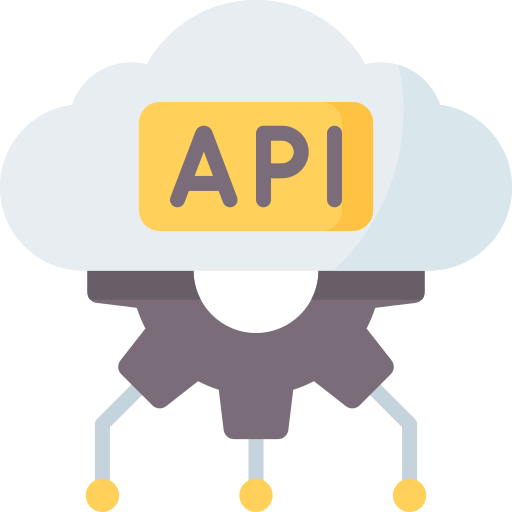
\includegraphics[height=1.5cm]{Figuras/api_logo.png}
    \caption{Servicios externos}
\end{figure}

\subsection{Integración y despliegue continuo}

El ciclo de vida del desarrollo se apoya en un flujo de integración y despliegue continuo mediante \textbf{GitHub Actions}, que automatiza la ejecución de pruebas y el despliegue del sistema tras cada cambio relevante en el repositorio.

El despliegue se realiza en la plataforma \textbf{Render}, integrada directamente con GitHub, lo que permite una actualización automática del entorno de producción. Esta decisión responde a criterios de viabilidad y gratuidad, adecuados al contexto académico del proyecto.

\begin{figure}[H]
    \centering
    
\includegraphics[height=1.5cm]{Figuras/github_logo.png}\hspace{1cm}
    
\includegraphics[height=1.5cm]{Figuras/render_logo.png}
    \caption{Tecnologías de integración y despliegue continuo}
\end{figure}

\subsection{Arquitectura global de la aplicación}

La arquitectura global sigue un enfoque modular y desacoplado, facilitando la escalabilidad, mantenibilidad y adaptación futura del sistema.

\tikzstyle{block} = [rectangle, draw, node distance=4.5cm,
    text width=6em, text centered, rounded corners, minimum height=3em, fill=blue!10]
\tikzstyle{line} = [draw, -latex']

\begin{figure}[H]
\centering
\begin{tikzpicture}
    \node [block] (Frontend) {Frontend \\ (Ionic + Angular)};
    \node [block, below of=Frontend, node distance=5cm] (Backend) {Backend REST \\ (Node.js + Express)};
    \node [block, below of=Backend, node distance=5cm] (DB) {Base de datos \\ (MongoDB)};
    \node [block, left of=Backend, node distance=7.2cm] (External) {Servicios externos};
    \node [block, right of=Backend, node distance=6.3cm] (CI) {CI/CD \\ (GitHub Actions + Render)};
    \path [line] ([xshift=-1.5mm]Frontend.south) -- node[left] {Solicitudes API} ([xshift=-1.5mm]Backend.north);
    \path [line] ([xshift=1.5mm]Backend.north) -- node[right] {Respuestas API} ([xshift=1.5mm]Frontend.south);
    \path [line] ([xshift=-1.5mm]Backend.south) -- ([xshift=-1.5mm]DB.north);
    \path [line] ([xshift=1.5mm]DB.north) -- ([xshift=1.5mm]Backend.south);
    \path [line] (Backend.west) -- (External.east);
    \path [line] (CI) -- (Backend);
    \path [line] (CI) to[bend right=20] (Frontend);
\end{tikzpicture}
\caption{Arquitectura global de la aplicación}
\end{figure}

Con esta arquitectura y selección tecnológica, el sistema satisface los requisitos funcionales y no funcionales definidos, garantizando su viabilidad técnica en un contexto académico y dejando abiertas futuras líneas de evolución hacia entornos de producción más exigentes.

\chapter{Planificación}

La planificación del proyecto se ha realizado con el objetivo de establecer una hoja de ruta clara y realista que permita organizar las tareas de forma secuencial y coordinada, facilitando así un seguimiento adecuado del progreso y la gestión del tiempo.

Se ha optado por un enfoque pragmático que prioriza la flexibilidad y adaptación a las circunstancias, sin ceñirse a una metodología de gestión específica. Esto permite ajustar las tareas y los plazos según las necesidades reales que vayan surgiendo durante el desarrollo, manteniendo un equilibrio entre el avance técnico y la calidad del resultado.

El cronograma elaborado refleja las fases principales del proyecto, divididiéndose en tareas y sub-tareas de manera que cada etapa se pueda abordar con foco y control, garantizando la coherencia y la continuidad del trabajo.

En resumen, la planificación establece un marco de referencia que orienta la ejecución del proyecto, pero deja espacio para la flexibilidad necesaria en un contexto académico y de investigación, donde el aprendizaje y la evolución del trabajo son parte fundamental del proceso.
\clearpage
\thispagestyle{fancy}
\begin{sidewaysfigure}
    \centering
    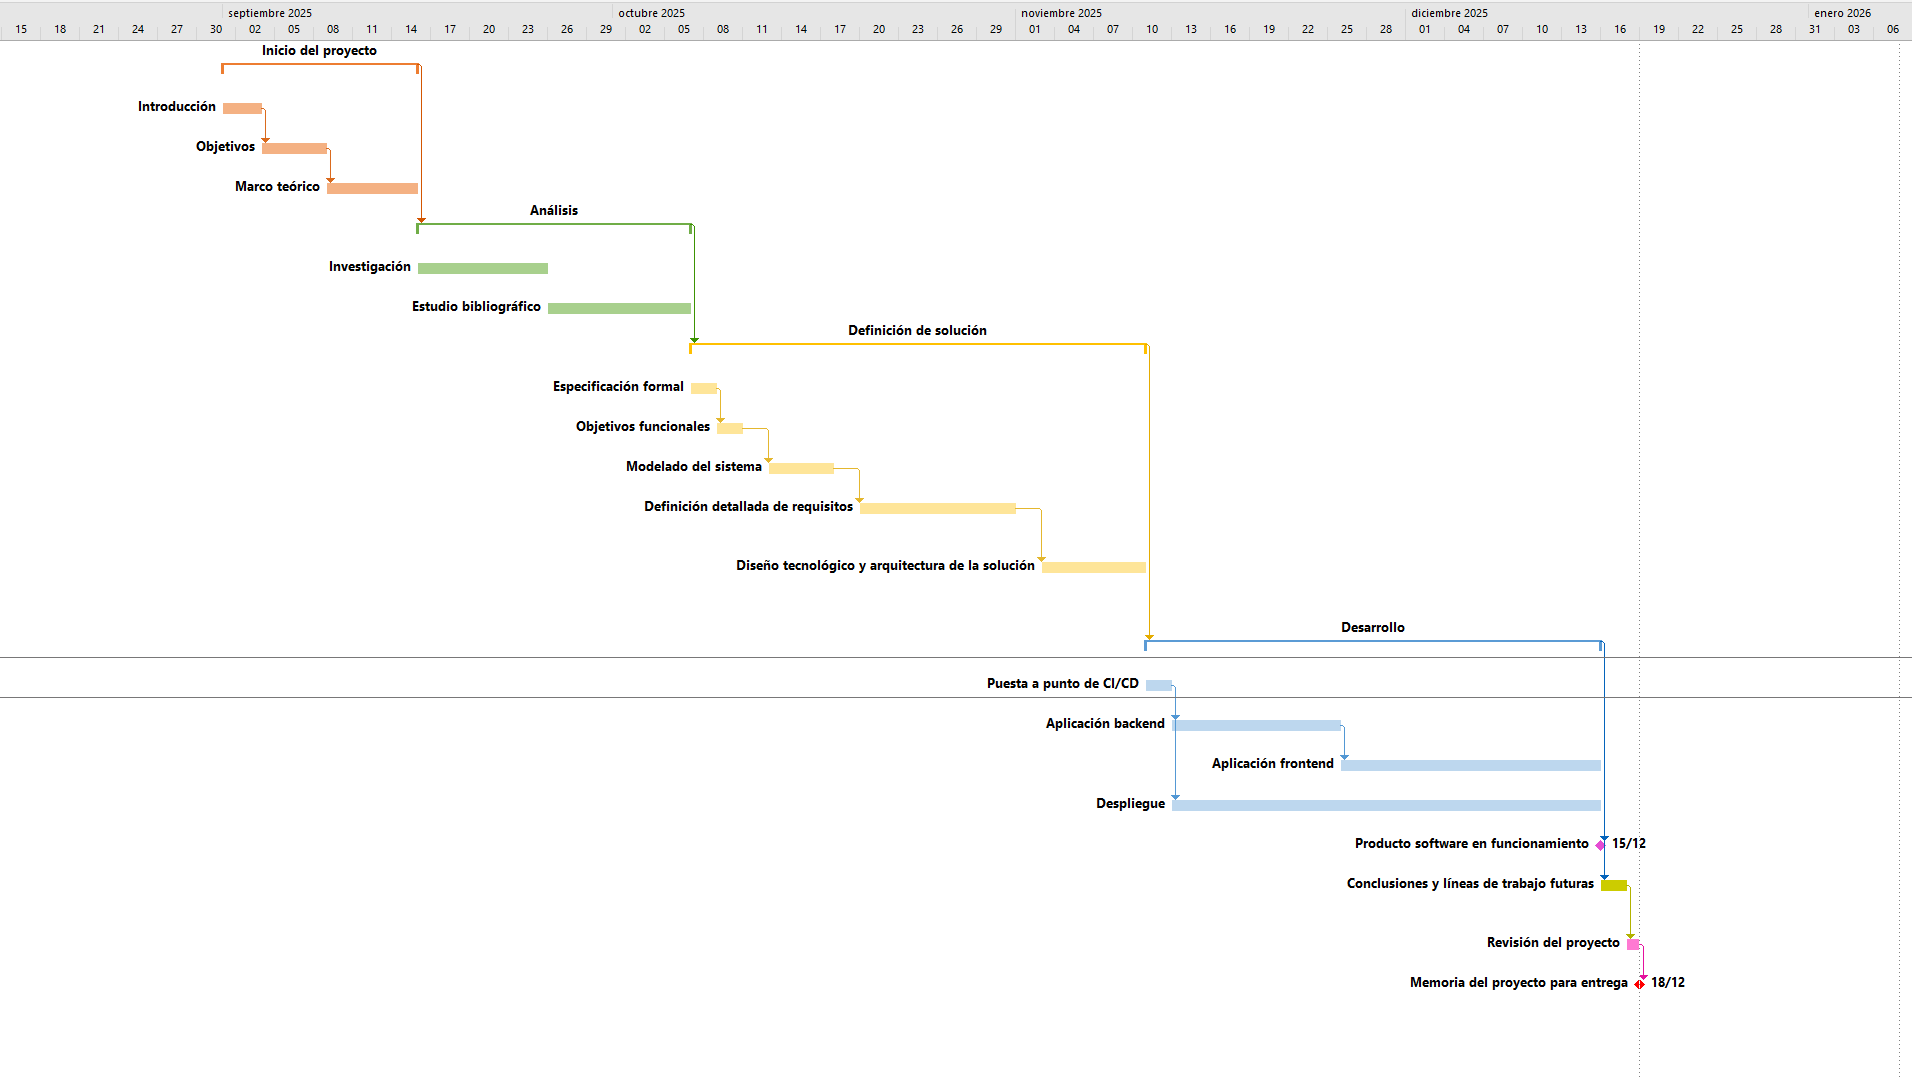
\includegraphics[width=\textwidth]{Figuras/cronograma.png}
    \caption{Cronograma del proyecto}
    \label{fig:cronograma}
\end{sidewaysfigure}
\clearpage

\chapter{Desarrollo de la aplicación backend}
\label{chap:backend}

En este capítulo se describe el proceso de desarrollo de la aplicación backend del sistema, que actúa como núcleo funcional encargado de gestionar la lógica de negocio, la persistencia de los datos y la comunicación con el frontend y con servicios externos. El backend proporciona una interfaz de acceso uniforme y segura a los recursos del sistema mediante una API REST, permitiendo una interacción desacoplada y escalable entre los distintos componentes de la aplicación.

Se presentan las decisiones de diseño adoptadas, la arquitectura y organización interna del backend, así como los mecanismos implementados para garantizar la seguridad, la calidad y la mantenibilidad del sistema.

\section{Arquitectura y visión general del backend}

La aplicación backend se ha diseñado siguiendo una arquitectura cliente-servidor basada en servicios REST, donde el servidor expone un conjunto de endpoints que permiten al frontend interactuar con los distintos recursos del sistema. Las comunicaciones se realizan mediante peticiones HTTP y respuestas en formato JSON, lo que facilita la interoperabilidad y la integración con otros posibles clientes o servicios externos.

Desde el punto de vista estructural, el backend adopta una separación de responsabilidades inspirada en el patrón Modelo-Vista-Controlador (MVC), adaptado al contexto de una API REST. Aunque no existe una capa de vista tradicional, el sistema diferencia claramente entre:
\begin{itemize}
    \item \textbf{Modelos}, responsables de definir la estructura de los datos, sus validaciones y la interacción con la base de datos.
    \item \textbf{Controladores}, que encapsulan la lógica de negocio y coordinan las operaciones sobre los modelos en respuesta a las peticiones recibidas.
    \item \textbf{Rutas}, que actúan como capa de exposición de la API, definiendo los endpoints disponibles y delegando el procesamiento de las peticiones en los controladores correspondientes.
\end{itemize}

Esta organización favorece un diseño modular y desacoplado, en el que cada componente cumple una función claramente definida. Como resultado, se facilita la mantenibilidad del código, la incorporación de nuevas funcionalidades y la realización de pruebas de forma aislada.

A nivel de proyecto, el backend se estructura en distintos módulos y directorios que reflejan esta separación, incluyendo carpetas específicas para modelos, controladores, rutas y middlewares. Esta disposición contribuye a una mayor claridad del código y a una gestión más eficiente del desarrollo, especialmente en proyectos de crecimiento progresivo.

La persistencia de los datos del sistema se gestiona mediante una base de datos documental, integrada directamente con el backend. Esta capa de persistencia permite almacenar y recuperar de forma eficiente la información relacionada con los distintos elementos del sistema, asegurando la coherencia de los datos y proporcionando una base sólida sobre la que se apoya la lógica de negocio de la aplicación. Los detalles concretos de la modelización y el acceso a los datos se abordan en los apartados posteriores dedicados a la implementación.
\section{Modelado de datos}

Con el objetivo de proporcionar una visión global de la estructura de la información manejada por el sistema, se ha elaborado un modelo conceptual de datos que identifica las principales entidades del dominio y las relaciones existentes entre ellas. Este modelo permite comprender de forma clara cómo se organiza la información dentro de la aplicación y sirve como referencia para la posterior implementación de la persistencia de datos en el backend.

Es importante destacar que el diagrama presentado no corresponde a un diagrama Entidad-Relación (ER) en sentido estricto. Dado que el sistema utiliza una base de datos documental (MongoDB), no resulta adecuado aplicar un modelado relacional tradicional ni imponer las restricciones propias de este tipo de bases de datos. En su lugar, se adopta un enfoque conceptual que refleja la estructura lógica de los datos y sus relaciones semánticas, independientemente de su implementación física.

El modelo se centra, por tanto, en representar las entidades principales del sistema y las asociaciones existentes entre ellas, como relaciones uno a muchos o muchos a muchos, sin detallar atributos específicos ni operaciones. Esta abstracción resulta especialmente adecuada en entornos NoSQL, donde la flexibilidad del esquema permite distintas estrategias de persistencia que se definen a nivel de implementación.

La Figura~\ref{fig:modelo_conceptual} muestra el modelo conceptual de datos del sistema, proporcionando una visión estructural que complementa la definición funcional y arquitectónica presentada en los apartados anteriores.

\begin{figure}[H]
    \centering
    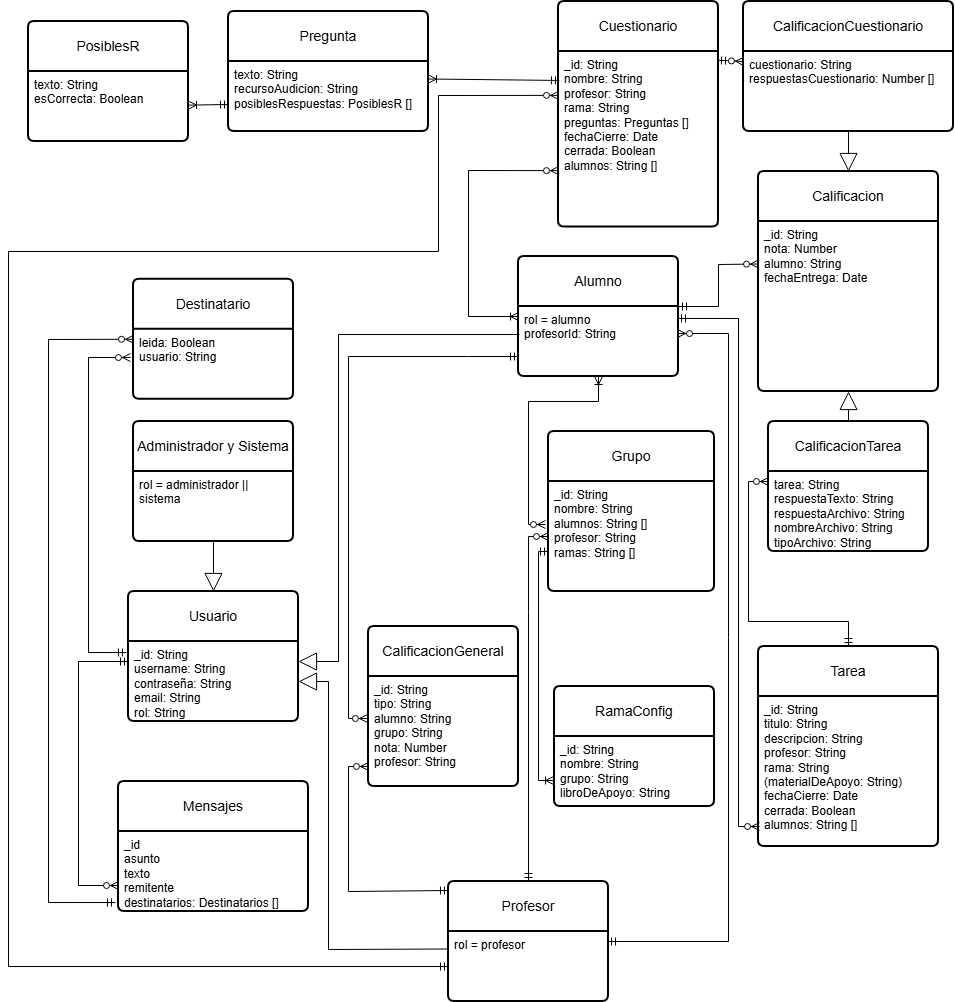
\includegraphics[width=\textwidth]{Figuras/modelo_Conceptual.png}
    \caption{Modelo conceptual de datos del sistema}
    \label{fig:modelo_conceptual}
\end{figure}
\section{Implementación de la lógica de negocio e integración}

En este apartado se describe la implementación de la lógica de negocio del backend, la integración con servicios externos y los mecanismos de seguridad y documentación que permiten garantizar la calidad, mantenibilidad y escalabilidad del sistema.

\subsection{Lógica de negocio: creación y actualización de calificaciones generales}

Un ejemplo representativo de la lógica de negocio es el método encargado de crear o actualizar calificaciones generales para los alumnos. Este método valida los datos de entrada, controla reglas específicas del dominio (como restricciones para calificaciones extraordinarias), maneja errores específicos y, además, genera un mensaje automático del sistema para notificar al alumno sobre la calificación.

\begin{verbatim}
exports.crearOActualizarCalificacionGeneral = async (alumnoId, grupoId, tipo, nota, profesorId) => {
    try {
        const validTypes = ['Q1', 'Q2', 'Q3', 'Ordinaria', 'Extraordinaria'];
        if (!tipo || !validTypes.includes(tipo)) {
            return { status: 400, body: { error: 'El tipo de calificación proporcionado no es válido.' } };
        }

        if (!validateNota(nota)) {
            return { status: 400, body: { error: 'La nota debe ser un número entero entre 1 y 10.' } };
        }

        const alumno = await Usuario.findById(alumnoId);
        if (!alumno || alumno.role !== 'alumno') {
            return { status: 400, body: { error: 'El ID de alumno proporcionado no es válido o el usuario no es un alumno.' } };
        }

        const grupo = await Grupo.findById(grupoId);
        if (!grupo) {
            return { status: 400, body: { error: 'El ID de grupo proporcionado no es válido.' } };
        }

        if (profesorId) {
            const profesor = await Usuario.findById(profesorId);
            if (!profesor || profesor.role !== 'profesor') {
                return { status: 400, body: { error: 'El ID de profesor proporcionado no es válido o el usuario no es un profesor.' } };
            }
        }

        if (tipo === 'Extraordinaria') {
            const ordinaria = await CalificacionGeneral.findOne({ alumno: alumnoId, grupo: grupoId, tipo: 'Ordinaria' });
            if (!ordinaria) {
                return { status: 400, body: { error: 'No se puede establecer una calificación Extraordinaria sin una calificación Ordinaria previa.' } };
            }
            if (ordinaria.nota >= 5) {
                return { status: 400, body: { error: 'Solo se puede establecer una calificación Extraordinaria si la calificación Ordinaria es menor de 5.' } };
            }
        }

        const calificacion = await CalificacionGeneral.findOneAndUpdate(
            { alumno: alumnoId, grupo: grupoId, tipo: tipo },
            { tipo: tipo, nota: nota, profesor: profesorId },
            { upsert: true, new: true, runValidators: true }
        );

        const sistemaUser = await Usuario.findOne({ username: 'sistema' });
        if (sistemaUser) {
            const asunto = `Calificación general de (${tipo})`;
            const texto = `La calificación obtenida en ${tipo} es ${nota}`;
            await mensajeController.crearMensaje(sistemaUser._id, asunto, texto, [alumnoId]);
        }

        return { status: 200, body: calificacion };

    } catch (error) {
        if (error.code === 11000) {
            return { status: 409, body: { error: `Ya existe una calificación de tipo '${tipo}' para este alumno en este grupo.` } };
        }
        if (error.name === 'ValidationError') {
            return { status: 400, body: { error: error.message } };
        }
        return { status: 500, body: { error: `Error al crear/actualizar la calificación: ${error.message}` } };
    }
};
\end{verbatim}

Este ejemplo muestra el manejo detallado de la lógica y validaciones propias del dominio, la interacción con la base de datos y la generación de mensajes del sistema para mantener informado al usuario.

\subsection{Integración con servicios externos}

Para funcionalidades específicas, como el envío de correos electrónicos, se integran servicios externos que simplifican el desarrollo y aseguran fiabilidad.

Por ejemplo, el siguiente método utiliza la API de Mailjet para enviar credenciales a un usuario nuevo:

\begin{verbatim}
export const enviarEmailCredenciales = async (destinatario, username, password) => {
  try {
    const request = mailjetClient.post('send', { version: 'v3.1' }).request({
      Messages: [
        {
          From: {
            Email: process.env.EMAIL_FROM,
            Name: process.env.EMAIL_FROM_NAME,
          },
          To: [
            {
              Email: destinatario,
              Name: username,
            },
          ],
          Subject: 'Tus credenciales para SolfEdge',
          HTMLPart: `
            <h1>¡Bienvenido a SolfEdge!</h1>
            <p>Hola ${username},</p>
            <p>Se ha creado una cuenta para ti en SolfEdge. A continuación encontrarás tus credenciales de acceso:</p>
            <ul>
              <li><strong>Usuario:</strong> ${username}</li>
              <li><strong>Contraseña:</strong> ${password}</li>
            </ul>
          `,
        },
      ],
    });

    await request;

    return { message: 'Correo enviado correctamente.' };
  } catch (err) {
    return {
      message: 'Error al enviar el correo.',
      error: err.statusCode ? `${err.statusCode} - ${err.message}` : err.message || JSON.stringify(err),
    };
  }
};
\end{verbatim}

Esta integración permite externalizar tareas complejas, aumentando la robustez y fiabilidad de la aplicación.

\subsection{Seguridad: autenticación mediante JWT}

La seguridad en el acceso a la API se implementa mediante tokens JWT, que se verifican con un middleware que protege las rutas del backend.

\begin{verbatim}
exports.verifyToken = (req, res, next) => {
    if (req.method === 'OPTIONS') {
        return next();
    }

    const authHeader = req.headers['authorization'];
    const token = authHeader && authHeader.split(' ')[1];

    if (!token) {
        return res.status(401).json({ error: 'Acceso denegado. No se proporcionó token.' });
    }
    const result = authController.verifySession(token);

    if (result.status === 200) {
        req.user = result.body.sessionData;
        next();
    } else {
        return res.status(result.status).json(result.body);
    }
};
\end{verbatim}

De esta forma, todas las rutas relevantes quedan protegidas, permitiendo solo el acceso a usuarios autenticados, salvo aquellas destinadas a usuarios no autenticados y la documentación de la API:

\begin{verbatim}
app.use('/api/auth', authRoutes);
app.use('/api-docs', swaggerUi.serve, swaggerUi.setup(swaggerSpec));

app.use('/api/usuarios', authMiddleware.verifyToken, usuarioRoutes);
app.use('/api/grupos', authMiddleware.verifyToken, grupoRoutes);
app.use('/api/mensajes', authMiddleware.verifyToken, mensajeRoutes);
app.use('/api/ramas', authMiddleware.verifyToken, ramaRoutes);
app.use('/api/tareas', authMiddleware.verifyToken, tareaRoutes);
app.use('/api/cuestionarios', authMiddleware.verifyToken, cuestionarioRoutes);
app.use('/api/calificaciones-generales', authMiddleware.verifyToken, calificacionGeneralRoutes);
app.use('/api/calificaciones', authMiddleware.verifyToken, calificacionRoutes);
\end{verbatim}

\subsection{Documentación de la API con Swagger}

Para facilitar la colaboración, mantenimiento y pruebas, la API está documentada con \textbf{Swagger}, que genera automáticamente una interfaz web interactiva accesible en la ruta \texttt{/api-docs}.

Esta documentación permite explorar los endpoints disponibles, con detalles sobre métodos, parámetros y respuestas, manteniendo la información siempre actualizada gracias a la sincronización con el código fuente.

\begin{figure}[H]
    \centering
    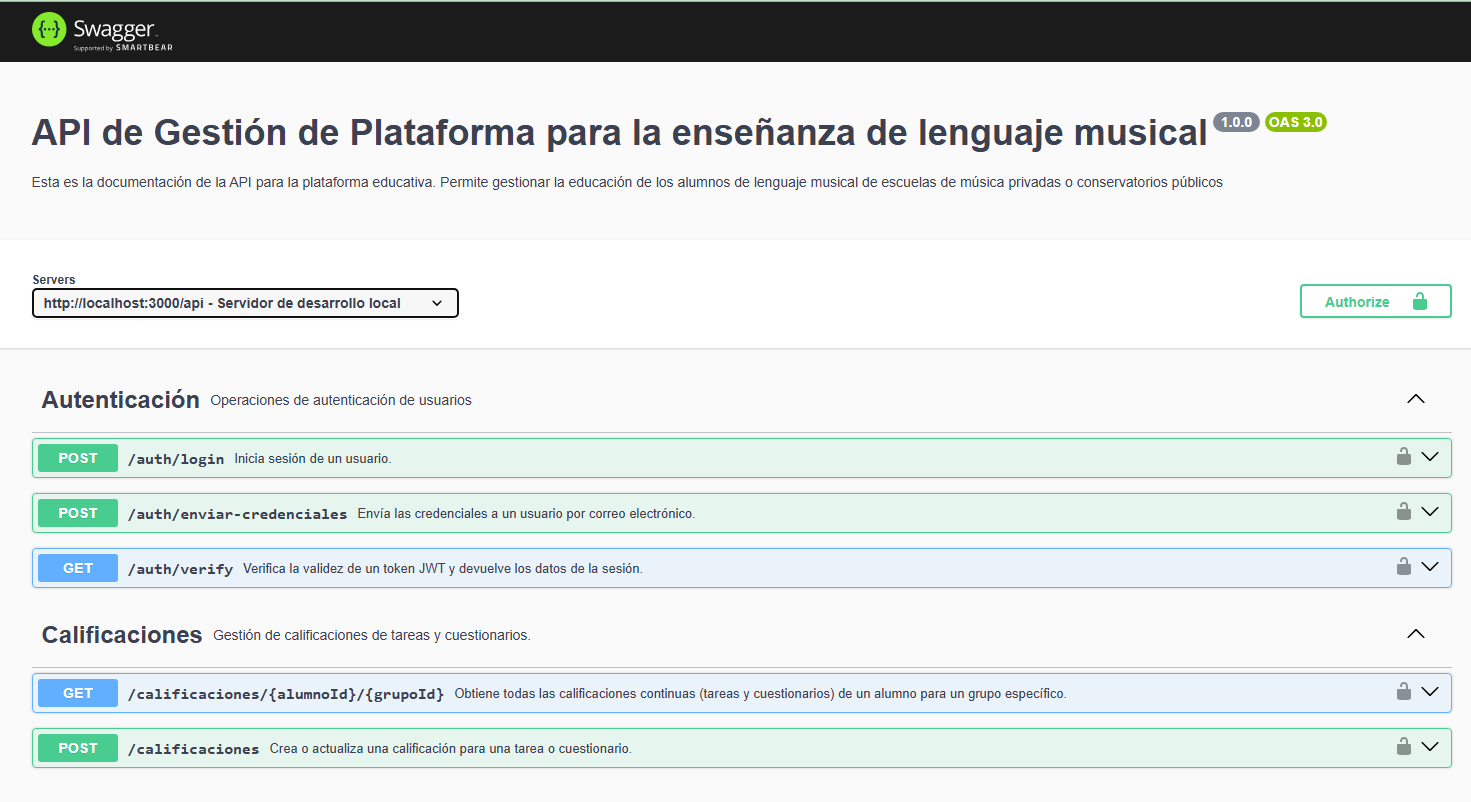
\includegraphics[width=0.9\textwidth]{Figuras/swagger_demo.png}
    \caption{Interfaz de la documentación generada por Swagger}
    \label{fig:swagger}
\end{figure}

Este enfoque mejora la mantenibilidad del sistema y simplifica la integración de nuevos desarrolladores o testers durante el ciclo de vida del proyecto.


Con esta estructura, la implementación del backend cubre desde la lógica de negocio hasta la seguridad y la documentación, garantizando un sistema robusto, seguro y fácil de mantener.
\section{Testing}

Para asegurar la calidad y fiabilidad del backend, se ha implementado un conjunto de pruebas automatizadas que abarcan diferentes niveles, con el objetivo de detectar errores tempranamente y facilitar el mantenimiento del código.

\subsection{Estrategia de pruebas}

El proceso de testing se basa en dos tipos principales de pruebas:

\begin{itemize}
    \item \textbf{Pruebas unitarias:} Se validan individualmente las funciones y métodos que componen la lógica de negocio y el acceso a datos, comprobando que cada unidad cumpla con el comportamiento esperado ante diversas situaciones.
    \item \textbf{Pruebas de integración:} Se verifican las interacciones entre distintos módulos y componentes del backend, incluyendo la comunicación con la base de datos y la integración con servicios externos, asegurando que el sistema funcione correctamente como conjunto.
\end{itemize}

\subsection{Herramientas utilizadas}

Se han utilizado herramientas especializadas que permiten automatizar y gestionar de forma eficiente las pruebas:

\begin{itemize}
    \item \textbf{Jest:} Framework para pruebas unitarias en JavaScript, que proporciona funcionalidades para mocks, aserciones y cobertura de código.
    \item \textbf{Supertest:} Herramienta para realizar pruebas sobre endpoints HTTP, facilitando la simulación de peticiones y validación de respuestas en la API REST.
\end{itemize}

\subsection{Ejemplo de prueba}

A modo ilustrativo, se presenta un ejemplo de prueba unitaria sobre la función que crea o actualiza una calificación general, comprobando tanto el resultado esperado como el manejo de errores:

\begin{verbatim}
    describe('POST /calificaciones-generales', () => {
        it('should create or update a general qualification', async () => {
            const mockCalificacion = {
                _id: 'calG1',
                alumno: 'alumno1',
                grupo: 'grupo1',
                tipo: 'Ordinaria',
                nota: 8,
                toObject: () => ({
                    _id: 'calG1',
                    alumno: 'alumno1',
                    grupo: 'grupo1',
                    tipo: 'Ordinaria',
                    nota: 8
                })
            };

            Usuario.findById
                .mockResolvedValueOnce({ _id: 'alumno1', role: 'alumno' })     // alumno
                .mockResolvedValueOnce({ _id: 'profesor1', role: 'profesor' }); // profesor

            Grupo.findById.mockResolvedValue({ _id: 'grupo1' });
            CalificacionGeneral.findOneAndUpdate.mockResolvedValue(mockCalificacion);
            Usuario.findOne.mockResolvedValue({ _id: 'sistema-user' });
            mensajeController.crearMensaje.mockResolvedValue({});

            const response = await request(app)
                .post('/calificaciones-generales')
                .send({
                    alumnoId: 'alumno1',
                    grupoId: 'grupo1',
                    tipo: 'Ordinaria',
                    nota: 8,
                    profesorId: 'profesor1'
                });

            expect(response.status).toBe(200);
            expect(response.body).toEqual(mockCalificacion.toObject());
        });
        it('should return 400 for invalid nota', async () => {
            const response = await request(app)
                .post('/calificaciones-generales')
                .send({ alumnoId: 'alumno1', grupoId: 'grupo1', tipo: 'Ordinaria', nota: 11, profesorId: 'profesor1' });

            expect(response.status).toBe(400);
            expect(response.body).toEqual({ error: 'La nota debe ser un número entero entre 1 y 10.' });
        });
        it('should return 400 if Extraordinaria is set without prior Ordinaria', async () => {
            Usuario.findById
                .mockResolvedValueOnce({ _id: 'alumno1', role: 'alumno' })
                .mockResolvedValueOnce({ _id: 'profesor1', role: 'profesor' });

            Grupo.findById.mockResolvedValue({ _id: 'grupo1' });
            CalificacionGeneral.findOne.mockResolvedValue(null);

            const response = await request(app)
                .post('/calificaciones-generales')
                .send({
                    alumnoId: 'alumno1',
                    grupoId: 'grupo1',
                    tipo: 'Extraordinaria',
                    nota: 6,
                    profesorId: 'profesor1'
                });

            expect(response.status).toBe(400);
            expect(response.body).toEqual({
                error: 'No se puede establecer una calificación Extraordinaria sin una calificación Ordinaria previa.'
            });
        });
        it('should return 400 if Extraordinaria is set with Ordinaria >= 5', async () => {
            Usuario.findById
                .mockResolvedValueOnce({ _id: 'alumno1', role: 'alumno' })
                .mockResolvedValueOnce({ _id: 'profesor1', role: 'profesor' });

            Grupo.findById.mockResolvedValue({ _id: 'grupo1' });
            CalificacionGeneral.findOne.mockResolvedValue({ nota: 5 });

            const response = await request(app)
                .post('/calificaciones-generales')
                .send({
                    alumnoId: 'alumno1',
                    grupoId: 'grupo1',
                    tipo: 'Extraordinaria',
                    nota: 6,
                    profesorId: 'profesor1'
                });

            expect(response.status).toBe(400);
            expect(response.body).toEqual({
                error: 'Solo se puede establecer una calificación Extraordinaria si la calificación Ordinaria es menor de 5.'
            });
        });
    });
\end{verbatim}
\section{Despliegue del backend}

El despliegue de la aplicación backend se ha realizado mediante un flujo automatizado de integración y despliegue continuo (CI/CD), configurado para garantizar la calidad, estabilidad y rapidez en las entregas.

Se utiliza \textbf{GitHub Actions} como herramienta principal para orquestar este pipeline, el cual incluye los siguientes pasos:

\begin{itemize}
    \item \textbf{Compilación:} Se verifica que el código fuente compile correctamente y cumpla con las configuraciones definidas.
    \item \textbf{Ejecución de pruebas:} Se ejecutan las pruebas unitarias e de integración desarrolladas con \textbf{Jest} y \textbf{Supertest}, validando la funcionalidad y fiabilidad del backend. Este paso es crucial para detectar fallos tempranos antes de proceder al despliegue.
    \item \textbf{Despliegue automático:} Una vez superadas las pruebas, el sistema se despliega automáticamente en el entorno de producción alojado en \textbf{Render}, asegurando que la última versión estable esté disponible para su uso.
\end{itemize}

Este proceso continuo aporta varios beneficios, entre ellos:

\begin{itemize}
    \item \textbf{Calidad constante:} Al ejecutar las pruebas en cada commit, se garantiza que el código desplegado cumple con los requisitos funcionales y no introduce regresiones.
    \item \textbf{Agilidad en las entregas:} La automatización reduce tiempos y riesgos asociados a despliegues manuales, facilitando iteraciones rápidas y confiables.
    \item \textbf{Transparencia y trazabilidad:} Cada paso del pipeline queda registrado y es accesible para revisión, lo que facilita la detección y solución de posibles incidencias.
\end{itemize}

\begin{figure}[H]
    \centering
    \includegraphics[width=0.85\textwidth]{Figuras/ci_cd_backend.png}
    \caption{Captura del pipeline de integración y despliegue continuo mostrando la ejecución exitosa de las pruebas unitarias e integración}
    \label{fig:ci_cd_backend}
\end{figure}

Este enfoque permite mantener un backend robusto y actualizado, alineado con las buenas prácticas actuales de desarrollo y despliegue de software.


%\chapter {Herramientas y entornos}
%\label{sec:herrra}

\chapter {Conclusiones y trabajo futuro}
\label{sec:conclu}